\documentclass[a4paper]{article}

\usepackage{amsmath}
\usepackage{amssymb}
\usepackage{parskip}
\usepackage{fullpage}
\usepackage{hyperref}
\usepackage{stellar}
\usepackage{chemfig}
\usepackage{bettelini}
\usepackage{tikz}
\usepackage{fancybox}
\usepackage{makecell}
\usepackage{wrapfig}

\usetikzlibrary{cd}

\hypersetup{
    colorlinks=true,
    linkcolor=black,
    urlcolor=blue,
    pdftitle={Biology},
    pdfpagemode=FullScreen,
}

\newcommand{\quotes}[1]{``#1''}

\newcommand\hr{\par\vspace{-.5\ht\strutbox}\noindent\hrulefill\par\vspace{0.15cm}}

\title{Biology}
\author{Paolo Bettelini}
\date{}

\begin{document}

\maketitle
\tableofcontents
\pagebreak

% 978 88 6364 9437 (trovato)
% 978 88 6364 9635
% 978 88 6364 9659

% Il tessuto nervoso dell’esempio è formato da milioni di cellule nervose interconnesse, chiamate neuroni.

\section{Definizioni}

\sdefinition{Cellula}{
    La \textit{cellula} è la più piccola unità funzionale degli esseri
    viventi. È delimitata da una membrana plasmatica
    che racchiude varie strutture, dette organuli cellulari.
}

\sdefinition{Organulo}{
    Un \textit{organulo} è una struttura racchiusa da una membrana che svolge
    una funzione specifica all'interno della cellula.
}

\sdefinition{Tessuto}{
    Un \textit{tessuto} è costituito da gruppi
    di cellule simili che svolgono
    una specifica funzione.
}

% pag 14
Tutte le specie viventi sono suddivise in tre grandi gruppi:
\textbf{eubatteri} (Bacteria), \textbf{archebatteri} (Archaea)
ed \textbf{eucarioti} (Eukarya).
I primi due domini, eubatteri e archebatteri, identificano due gruppi di organismi
unicellulari molto diversi formati da cellule
procariote.
Il dominio degli eucarioti, invece, comprende or ganismi sia unicellulari
sia pluricellulari costituiti da cellule eucariote ed è,
a sua volta, suddiviso in più regni: \textbf{protisti},
\textbf{piante}, \textbf{funghi} e \textbf{animali}.

\pagebreak

\section{Sistemi}

\sdefinition{Sistema}{
    Un \textit{sistema} (vivente e non-vivente) è composto di parti differenti, specializzate e interdipendenti. 
    
    \begin{enumerate}
        \item Organizzazione della relazione fra le parti
        \item Struttura fisica, chimica etc. 
        \item Processo di riproduzione
    \end{enumerate}
}

\sdefinition{Emergenza Sistemica}{
    Una \textit{emergenza sistemica} è lo scopo che le diverse parti riescono a raggiungere ed eseguire.
}

L'emergenza sistemica stabilisce anche delle relazioni materiali, energetiche e/o informazionali con l'esterno, cioè con l'ambiente.

\sdefinition{Molecola organica}{
    Una \textit{molecola organica} è una molecola che contiene in generale il carbonio (e.g tranne CO\({}_2\)).
}

\subsection{Sistemi viventi}

\sdefinition{ATP}{
    ATP è un composto organico che provvede energia alle cellule per le loro funzioni.
}

I seguenti processi sono eseguiti da tutti gli organismi viventi.

\textbf{Nutrizione:}
Tutti gli organismi viventi si nutrono con del \quotes{cibo}, ossia materia.
In generale, gli esseri viventi necessitano di \(C\), \(O\), \(H\), \(N\), \(S\) e \(P\).
L'unico nutrimento della pianta è CO\({}_2\) (materia inorganica), mentre
i nutrimenti degli animali sono materia organica.

\sdefinition{Autotrofo}{
    Un organismo \textit{autotrofo} può svolgere la propria funzione di nutrizione,
    elaborando alimenti inorganici mediante assunzione d'energia dal mondo inorganico.
}

\sdefinition{Eterotrofo}{
    Un organismo \textit{eterotrofo}
    si nutre di sostanze organiche prodotte dagli organismi autotrofi.
}

\textbf{Respirazione:}

Tutti gli organismi viventi respirano
\[
    C_6H_{12}O_6 + O_2 \rightarrow CO_2 + H_2O
\]
In assenza di ossigeno (si usa la materia organica per produrre energia), e alcuni organismi \textit{fermentano}.
Nel caso degli umani i muscoli respirano, se non c'è \(O\) fermentano e producono acido lattico
che deve successivamente essere smaltito.

Le piante respirano mediante la fotosintesi
\[
    CO_2 + H_2O \rightarrow C_6H_{12}O_6 + O_2
\]

\textbf{Si riproduce e ha un ciclo vitale}

\textbf{Evolve}

\textbf{È sensibile (sa rispondere all'ambiente)}

\textbf{Mantiene stabili le sue condizioni interne}

\sdefinition{Biotico}{
    Con \textit{biotico} si intende tutto ciò che è vivente o era vivente.
} % foglia morta, elefante

\sdefinition{Abiotico}{
    Con \textit{abiotico} si intende tutto ciò che non è vivente e non lo è mai stato.
} % roccia

\sdefinition{Detrito}{
    Con \textit{detrito} si intende il resto di ogni organismo vivente che è morto.
} % foglia morta

Il sistema vivente presenta le medesima ma caratteristiche del sistema non-vivente,
ma possiede anche le seguenti componenti.

\sdefinition{Componente}{
    Insieme di materia, concreta e tangibile
}

\sexample{Components}{
    Acqua, suolo, sali minerali, ossigeno.
}

\sdefinition{Fattore}{
    Derive dalla presenza di componenti, produce un determinato effetto o risultato e si può misurare.
}

\sexample{Fattore}{
    \begin{itemize}
        \item Decomposizione (fattore biotico).
        \item Predazione, catena alimentare (fattore biotico).
        \item Vento (fattore abiotico).
        \item Luce solare (fattore abiotico).
        \item Luce della lucciola (fattore biotico).
    \end{itemize}
}

Un fattore rappresenta tutto ciò che si può misurare e che non è una componente.

Ogni essere vivente possiede \underline{autopoiesi}, \underline{dissipazione} e \underline{cognizione.}

\subsubsection{Autopoiesi}

\sdefinition{Autopoiesi}{
    La capacità di ripararsi, modificarsi e riprodursi da solo, internamente ed in maniera autonoma.
}
I sistemi viventi sono organizzativamente chiusi, per cui hanno un confine.

\pagebreak

\textbf{Sistema autopoietico (ciclo):}
\begin{figure}[ht]
    \centering
    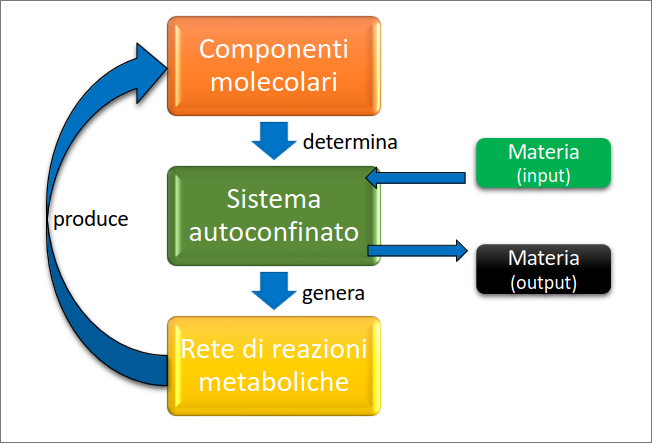
\includegraphics[width=0.65\textwidth]{./sis_autop_ciclo.png}
\end{figure}

\textbf{Sistema autopoietico (cellula):}
\begin{figure}[ht]
    \centering
    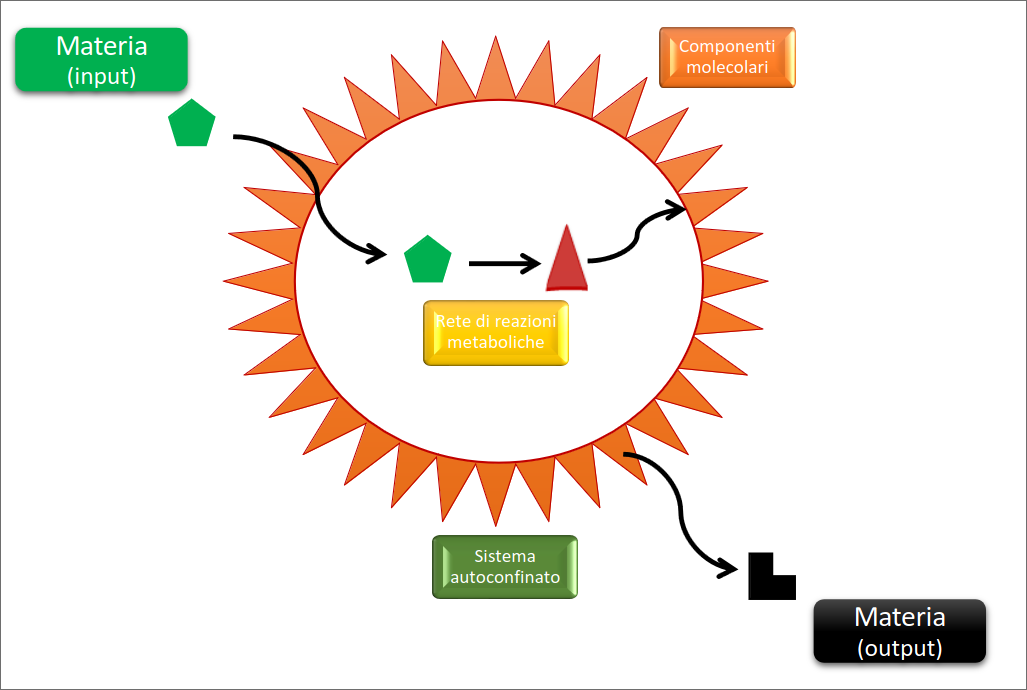
\includegraphics[width=0.65\textwidth]{./sis_autop_cellula.png}
\end{figure}

\subsubsection{Dissipazione}

\sdefinition{Dissipazione}{
    La necessità di consumare energia, materia ed informazioni dall'esterno.
}
I sistemi viventi sono metabolicamente aperti, per cui hanno degli scambi con l'esterno
e rinnovano il proprio materiale.

\subsubsection{Cognizione}

\sdefinition{Cognizione}{
    L'attiva conoscenza dell'ambiente, esterno ed interno, da parte del sistema.
}

\pagebreak

\section{Biomolecole}

\sdefinition{Biomolecola}{
    Le \textit{biomolecole} sono le molecole dei processi biologici degli essere viventi.
}

Tutte le biomolecole contengono \(C\), \(O\) e \(H\).
Ci sono delle eccezioni, per esempio, gli idrocarburi contengono solamente \(C\) e \(O\).

Le biomolecole sono di 4 tipi:
\begin{itemize}
    \item Lipidi (grasso)
    \item Acidi nucleici (DNA e RNA)
    \item Carboidrati
    \item Proteine
\end{itemize}

Le macromolecole sono composte da \textit{monomeri} e \textit{polimeri}.
Nel corpo umano i polimeri sono creati dalle cellule mediante alle istruzioni nel DNA.
Le biomolecole fanno dei polimeri.

\sdefinition{Isomero}{
    Gli \textit{isomeri} sono delle molecole distinte con il medesimo numero di atomi,
    ma con una struttura diversa. Diversi isomeri potrebbero avere proprietà diverse.
}

\paragraph{Costruzione di polimeri}

Tutti i monomeri posseggono, da una parte un gruppo di idrogeno \(H\),
e dall'altra un gruppo \(OH\).
Due monomeri si uniscono mediante una reazione chimica chiamata \textit{condensazioe} o \textit{disidratazione}, la quale consiste
nell'unire un'estremità \(H\) con una \(OH\) mediante un legame.
La condensazione libera una molecola d'acqua come scarto.

\paragraph{Disintegrazione di polimeri}

Per separare un legame fra due monomeri, viene utilizzata la reazione chimica di \textit{idrolisi} o \textit{idratazione}.
Questa reazione necessita di una molecola di \(H_2O\).

\pagebreak

\subsection{Carboidrati}

\sdefinition{Carboidrato}{
    I \textit{carboidrati} sono dei tipi di biomolecole composti da carbonio, idrogeno e ossigeno
    \((CH_2O)_n\).
}

I monomeri di carboidrati si chiamano monosaccaridi.
I polimeri di carboidrati si chiamano polisaccaridi (disaccaridi, trisaccaridi)

\sdefinition{Maltosio}{
    Il \textit{maltosio} è composto da due molecole di glucosio (\(C_{12}H_{22}O_{11}\)).
}

Per unire 2 molecole di glucosio
è necessario perderne una di \(H_2O\). Per cui il maltosio è dato da \(C_{12}H_{22}O_{11}\).

\sdefinition{Saccarosio}{
    Il \textit{saccarosio} è composto da un glucosio e un fruttosio (\(C_{12}H_{22}O_{11}\)).
}
\sdefinition{Lattosio}{
    Il \textit{lattosio} è composto da un glucosio e un galattosio (\(C_{12}H_{22}O_{11}\)).
}

I monosaccaridi sono glucosio, fruttosio, galattosio (isomeri).

\sdefinition{Amido}{
    L'\textit{amido} è un polisaccaride che viene prodotto dalle piante.
    Esso è composto da una catena di glucosi arrotolati ad elica.
}

L'\textit{amilasi} è l'enzima che rompe l'amido.
Esso fa parte della famiglia degli \textit{idrolasi}, ossia tutti gli enzimi che
eseguono l'idrolisi.

\sdefinition{Glicogeno}{
    Il \textit{glicogeno} è un polisaccaride che viene prodotto dagli animali.
    Esso è composto da diverse diramazioni di catene di glucosio.
}

Amido e glicogeno occupano meno spazio dei monomeri da soli, per cui sono ottimali per immagazzinare
il glucosio.

Gli esseri umani immagazzinano il glucosio in eccesso nei muscoli e nel fegato, dove ci sono degli enzimi
che sono in grado di creare questi polimeri di glucosio.

\sdefinition{Cellulosa}{
    La \textit{cellulosa} è un polisaccaride di glucosio prodotto dalle piante.
    Esso è composto un insieme di fibre lineari.
}

La cellulosa serve per dare rigidità al tessuto delle piante.

I polisaccaridi sono amido, glicogeno e cellulosa.

% Sintesi dello sciroppo di mais

\pagebreak

\subsection{Proteine}

I monomero di proteine si chiamano \textit{amminoacidi}.

% TODO foto

Ci sono 20 possibili amminoacidi diversi.

\sdefinition{Catena Polipeptidica}{
    Una \textit{catena polipeptidica} è una catena di amminoacidi.
}

\sdefinition{Proteina}{
    Le \textit{proteine} sono delle biomolecole costruite
    da una o più catene polipeptidiche.
}

Le proteine si distinguono in 7 classi per funzione
\begin{enumerate}
    \item \textbf{Strutturali:} es. unghie (cheratina).
    % Elastina, Collagene

    \item \textbf{Contrattili:} costituiscono il muscolo.
    % Actina e Miosina

    \item Di \textbf{riserva:} costituiscono una riserva di amminoacidi (specialmente per l'embrione).
    % Es. Albumina, Caseina

    \item Di \textbf{difesa:} costituiscono gli anticorpi, neutralizzano gli agenti patogeni.
    
    \item Di \textbf{trasporto:} trasportano l'ossigeno all'interno del sistema circolatorio.
    % Emoglobina

    \item \textbf{Regolatrici:} costituiscono alcuni ormoni.
    % Insulina

    \item \textbf{Enzimi:} costituiscono gli enzimi.
\end{enumerate}

\pagebreak

\subsection{Lipidi}

\sdefinition{Lipido}{
    I \textit{lipidi} sono un insieme di molecole idrofobe.
}

I lipidi non sono strutturati con monomeri e polimeri.

I lipidi vengono categorizzati nelle seguenti classi:

\subsubsection{Trigliceride}

\sdefinition{Trigliceride}{
    Il \textit{trigliceride} è una riserva energetica della cellula (comunemente grasso).
}

Il monogliceride è composto da un glicerolo, attaccato (per condensazione) ad un acido grasso.
Il trigliceride è attaccato a 3 catene di acido grasso.

Le catene di acidi grassi possono essere dritti (saturi) oppure piegate (insaturi).
Alle catene insature mancano alcuni doppi legami.

\subsubsection{Fosfolipide}

\sdefinition{Fosfolipide}{
    Il \textit{fosfolipide} sono composti da una testa idrofila e da una code idrofoba.
}

Le catarriteristiche idrofobe e idrofile permettono ai fosfolipidi di disporsi in maniera ordinata,
con la testa verso l'acqua e la coda rivolta verso l'esterno.

\subsubsection{Steroidi}

\sdefinition{Steroide}{
    Lo \textit{steroide} è una molecola con una struttura di 4 anelli.
}

Alcuni esempi sono il colesterolo, testosterone ed estrogeno.

\pagebreak

\subsection{Acidi nucleici}

I monomeri degli aicid nucleici si chiamano \textit{nucleotidi}.
% polimero = acido nucleico
\sdefinition{Acido nucleico}{
    L'\textit{acido nucleico} è composto da un gruppo fosfato, zucchero e base azotata.
}

\sdefinition{DNA}{
    Il \textit{DNA} è composto da due filamenti di nucleotidi.
}

I nucleotidi del DNA sono 4 (A, C, G, T).

\pagebreak

\section{Bioenergetica}

\subsection{Le membrane}

\sdefinition{Membrana}{
    Le membrane sono dei fosfolipidi con una code e una testa idrofila.
}

Questi fosfolipidi si attraggono per polarità e possono formare le seguenti composizioni

\begin{figure}[h]
    \centering
    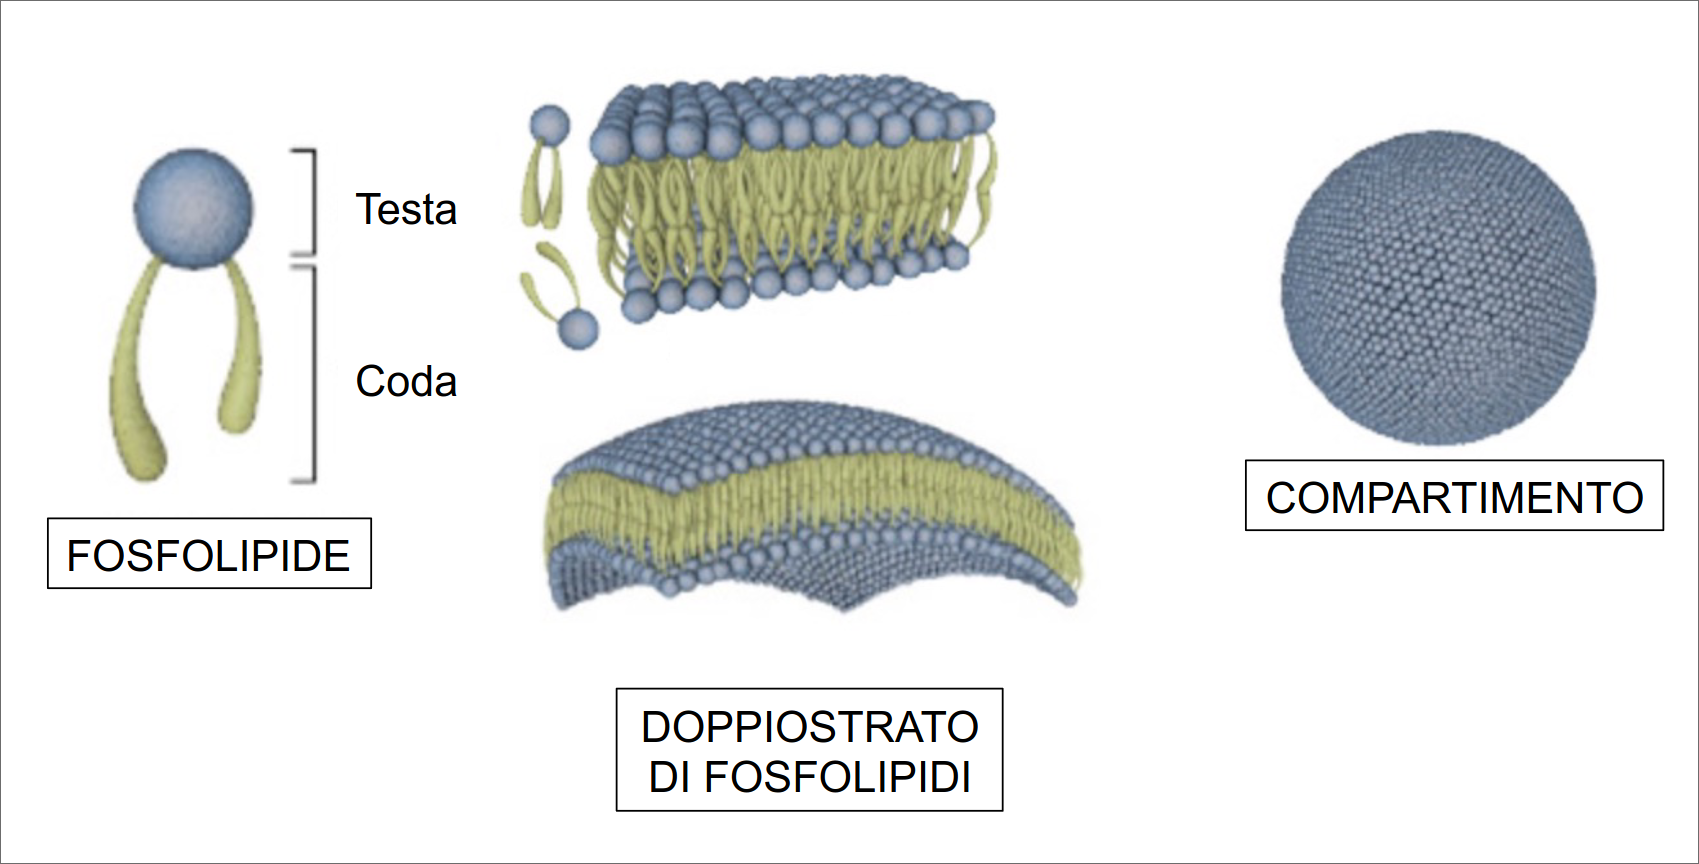
\includegraphics[width=\textwidth]{./membrana.png}
\end{figure}

Le sostanze idrofile (steroidi, grassi, etc.) vengono trasportati nel sangue

\subsubsection{Proteine di membrana}

\sdefinition{Gradiente di concentrazione}{
    Il \textit{gradiente di concentrazione} è un regolare incremento o diminuzione della concentrazione di una sostanza. Quando è presente un gradiente di concentrazione, gli ioni o le altre sostanze coinvolte tendono a muoversi spontaneamente dalla zona di concentrazione maggiore a quella di concentrazione minore.
}

Le principali tipologie di proteine che vengono incastrate nelle membrane sono:
\sdefinition{Proteina di trasporto}{
    Una \textit{proteina di trasporto} (canale) è una proteine di membrana che forma un tunnel sempre aperto.
}
Ogni canale non è direzionale ed ogni canale è specifico per un certo soluto.

\begin{figure}[h!]
    \centering
    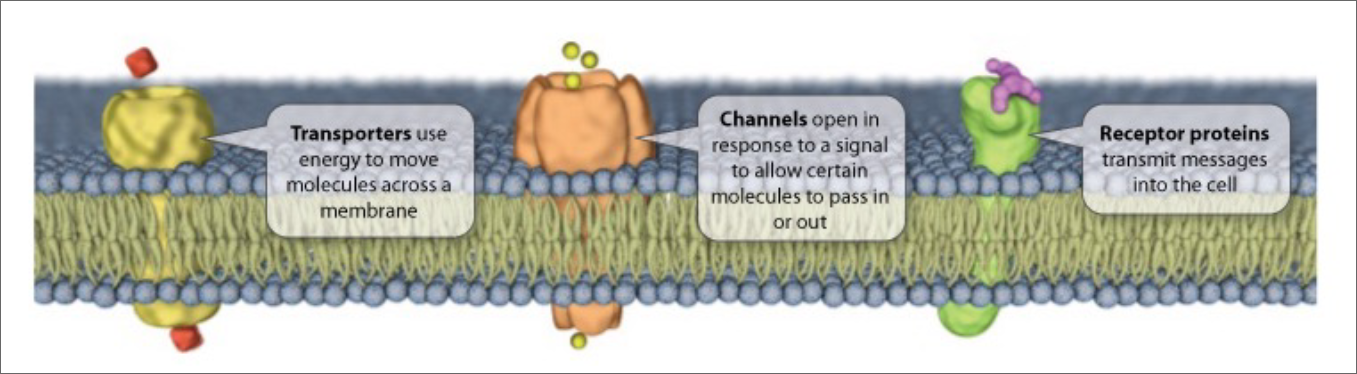
\includegraphics[width=\textwidth]{./proteine_mem.png}
\end{figure}

Tuttavia, siccome le cellule necessitano un ambiente interno diverso da quello esterno,
devono andare contro il gradiente di concentrazione.
Per risolvere questo problema vengono utilizzati i trasportatori.

\sdefinition{Trasportatore}{
    Un \textit{trasportatore} è una proteina che sposta una sostanza contro il gradiente.
}
Ogni tipo di trasportatore è specifico ad un tipo di sostanza.
Il trasportatore sposta quindi una sostanza da dove ce n'è poca a dove ce n'è tanta (mediante energia).

\sdefinition{Ricettori}{
    Un \textit{ricettore} è una proteina che comunica dei messaggi alla cellula.
}

\sexample{Ricettori}{
    Un ricettore potrebbe per esempio comunicare il segnale della presenza di un agente patogeno.
}

% todo fare 2 definitions
Alcune molecole possono passare direttamente attraverso la membrana, come per esempio l'azoto, l'ossigeno, acqua e glicerolo.
Questo movimento è detto diffusione semplice nei fosfolipidi. Chiaramente, la cellula non può controllare queste sostanze.

Le molecole grandi e ioni non passano per i fosfolipidi senza un canale (diffusione facilitata).

% grandiente elttrochimico con polarità

\sdefinition{Trasporto attivo primario}{
    Il \textit{trasporto attivo primario} è un trasporto grazie ad un trasportatore e all'ATP.
}

Se non viene utilizzata direttamente l'ATP,
bensì viene sfruttata la differenza di gradiente di concentrazione stabilita da un trasporto primario,
si parla di trasporto \textit{secondario}.

\sdefinition{Trasporto secondario}{
    Il \textit{trasporto secondario} sfrutta il gradiente di concentrazione per trasportare
    senza costo.
}

\begin{itemize}
    \item \textbf{Uniporto:} consente il passaggio di un solo ione o molecola in un'unica direzione.
    \item \textbf{Antiporto:} consente il passaggio contemporaneo ma in direzioni opposte di due ioni e/o molecole differenti2
    \item \textbf{Simporto:} consente il passaggio contemporaneo ma nella stessa direzione di due ioni e/o molecole differenti.
\end{itemize}

\subsubsection{Trasporto vescicolare}

Quando le molecole sono troppo grandi (es. proteine intere) per passare per un canale, possono essere trasportate 
mediante una \textit{vescicola di trasporto}. Il processo di entrata si chiama \textit{endocitosi},
mediante quello di uscita si chaima \textit{esocitosi}. 
In questa \href{https://youtu.be/uYpNUw7vPO4}{illustrazione} il colore blu rappresenta il contenuto di un organello.

\pagebreak

\subsubsection{Glucotrasportatori di membrana (Glut4)}

Gli enterociti prendono il glucosio e il Na\({}^+\) dal lume intestinale
e li trasportano fino al sangue grazie a un simporto Na\({}^+\)/glucosio, una glucosio permeasi
(una proteina per la diffusione facilitata del glucosio), e la Na\({}^+\)/K\({}^+\)ATPasi. 

\sdefinition{Endocitosi}{
    L'\textit{encodictosi} è un processo che le cellule utilizzano per l'assunzione di sostanze presenti nell'ambiente extracellulare o aderenti alla membrana della cellula stessa.
}

\begin{figure}[h]
    \centering
    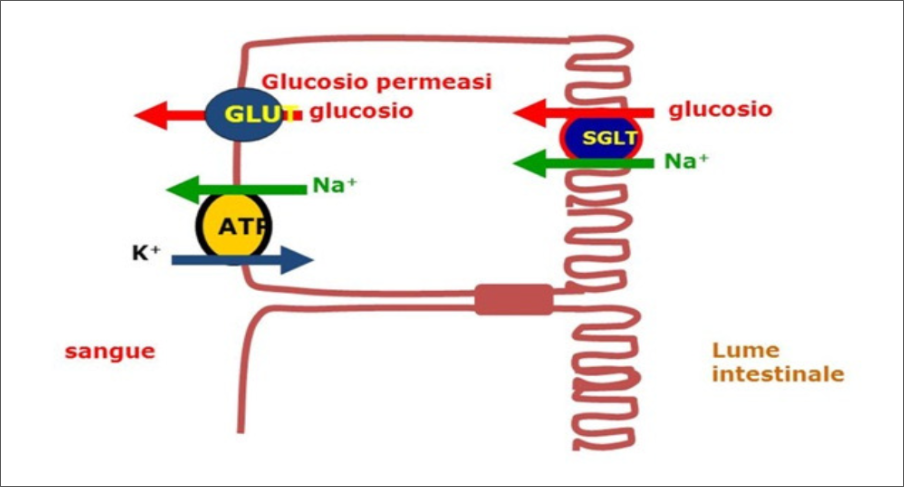
\includegraphics[width=\textwidth]{./glut4.png}
\end{figure}

I Glut4 verranno inseriti nella cellula quando il sangue è pieno di glucosio (quando la \textit{glicemia} è alta).
È necessario che la cellula risponda alla alta glicemia nel sangue per produrre i Glut4,
questo messaggio viene spedito attraverso il sangue con l'\textit{insulina}.
L'insulina lega il ricettore, cambiandone la struttura. \\
L'insulina viene prodotta dal pancreas, infatti, le cellule del pancreas sono in grado di misurare la glicemia.
    
\begin{figure}[h]
    \centering
    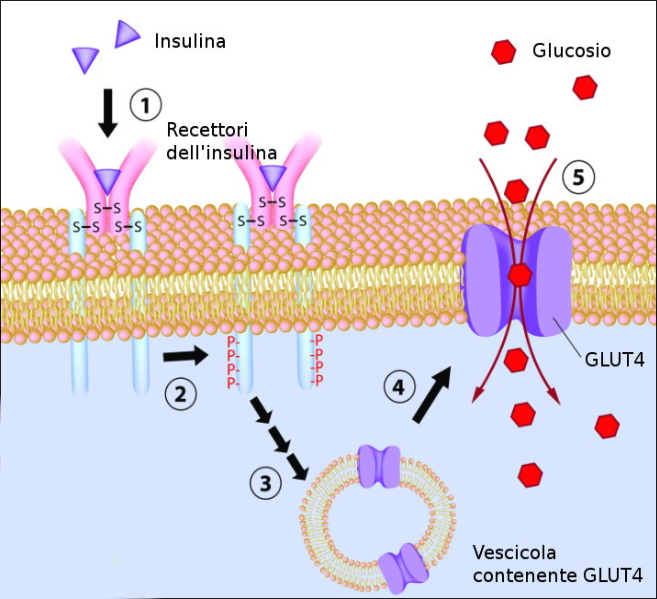
\includegraphics[width=0.5\textwidth]{./insulin.png}
\end{figure}

Il diabete è un problema nella ricezione dell'insulina.

\sdefinition{Omeostasi}{
    L'\textit{omeostasi} è il processo di autoregolazione dei vari valori.
}

Il seguente diagramma illustra un esempio di omeostasi per la regolazione della glicemia nel sangue.

\begin{figure}[h]
    \centering
    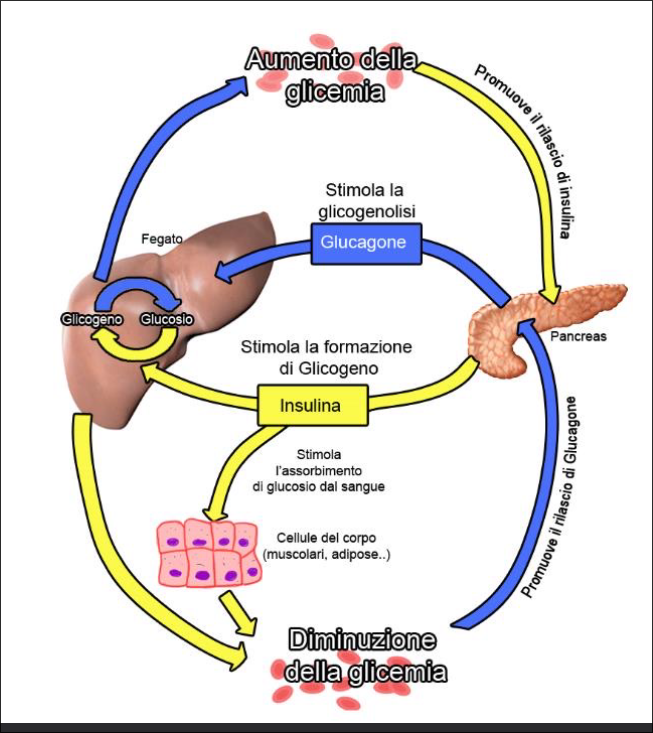
\includegraphics[width=0.6\textwidth]{./omeostasi.png}
\end{figure}

% https://tikzcd.yichuanshen.de/#N4Igdg9gJgpgziAXAbVABwnAlgFyxMJZAFgBoBGAXVJADcBDAGwFcYkQAdDnGADxwBGAM2ABBHHloQAviGml0mXPkIoAbBWp0mrdlx79hwAAr042KbPmLseAkQDMpAExaGLNok7c+OEwCcsAFt6QIgAAgAKUQAVYwBKKwUQDFsVIgBWFzcdT28DPwBlGABjAihQ-CSbZXsUMgccjz0ffmAAVTAsDH8cGTlk1NrVZCzGmnddL31fYELgnr7qlKU7EY1x7Wbp1r9RMDxF-usVtLrkDWImqZABmrXM0iuJ3PY70+GiMmetm-ehh4oAAcmhe23yswAIlghEJmNgCDBlgD0igAJzZME3GZtYpBNCMLAlJH-Vao5AAdkxvzyOL8ADF6CUsIScPQ2ciyecqZtJrTdsASvQwEwsJyziMMbzXjsCsAgjAggJ-ML6OLPvVSAAGa78gpGGIquCLMWkiVEZygmktfUiABq8GZZUYoRJJxR53I2t1NtmAFEwFAIMy+th1YDkF7XFi9f64MHcEpw+StVa+b62gBxFWBrDhND+CA8LBgN2DLkjL3S8F03DAP1wAB04Wk4TpwEzLBwxCsWhgUAA5vAiKAhIWgkhUyA+khnCcxxAJ4gpzPEA55+OkE5pxAkD3kgul9vVxkN4utzRV2oz0uNDukFSQAIYIGkABaBxam8Py+7xB359X0QD8vwPTdECye9EBBEBCVLdh40JKAQBoAALGB6GQxAwGYRhGEvegWXYSB4JoQCsKnOBUJhHAkHIb9EDIKC0QY8gVz-ch6LA89EDY386Lnbil3IS0oPIdchLor0xP3UdwPISDVynF1n0YYwK3YQIB1Q2iYwzPwAGECBwQtwmzTCsBfHhlkPOjFI4siXywz89NlWZjBgfwzJVKBLIOEkaBUmA1I0rwtJ095bN4+y6IApz30-Vi71XcgKSS-jeKBViMTEu84LyCoqP7FDp0Ixh2DZIi0IwrDpwAdwgdDMIQBjnHY2LHKAkDApLAqix4ZDAvoVT1PNLwS2wWASvTNzDBENAzAsY5JN4jK2IY48-1EmaITaOAx2YCQ1RK-L2CDCRioYmLoM6iiaComj33oyhpCAA
\begin{figure}[h]
    \centering
    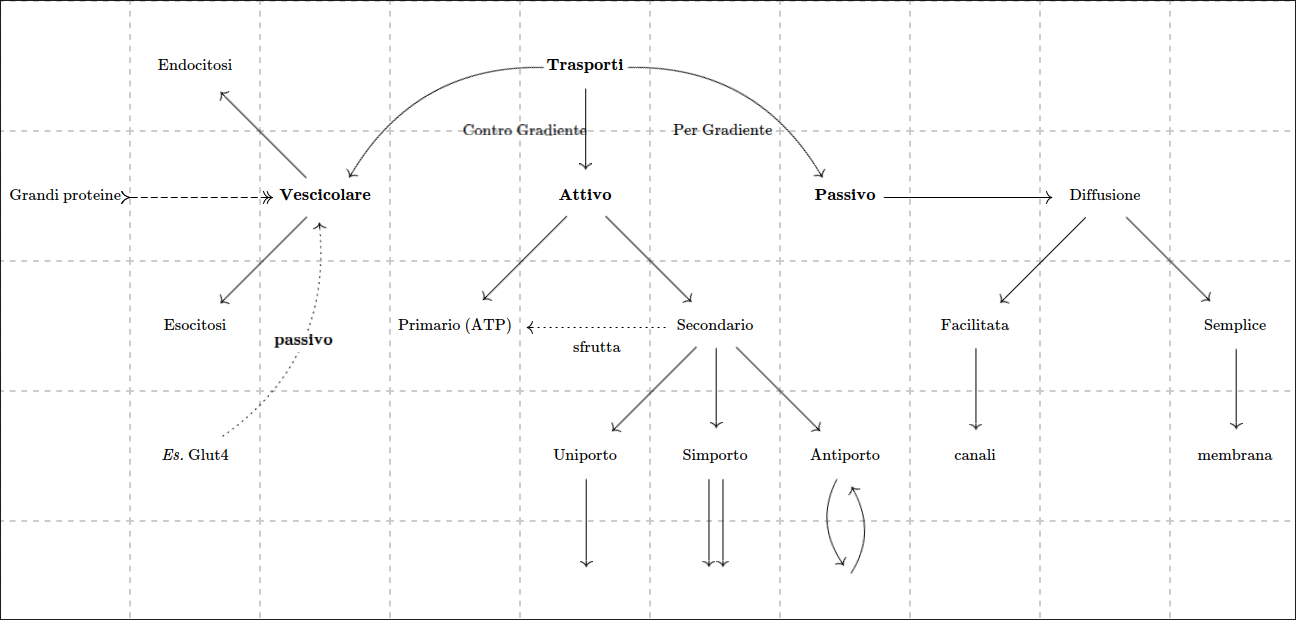
\includegraphics[width=\textwidth]{./schema.png}
\end{figure}

\pagebreak

\subsection{Reazioni tra enzimi e vie metaboliche}

\sdefinition{Enzima}{
    Gli \textit{enzimi} sono dei catalizzatori per aumentare le tempistiche delle varie reazioni chimiche.
}

\sdefinition{Metabolismo}{
    Il \textit{metabolismo} è l'insieme di tutte le reazioni chimiche nel corpo, catalizzate da un enzima.
}

\begin{center}
    % https://tikzcd.yichuanshen.de/#N4Igdg9gJgpgziAXAbVABwnAlgFyxMJZABgBpiBdUkANwEMAbAVxiRAB12cYAPHYAIIBfEENLpMufIRQBGclVqMWbTtz7AAQiLETseAkQBMC6vWatEHLr34BhHeJAZ90ogGZTSi6psaAIjqKMFAA5vBEoABmAE4QALZIZCA4EEjy3ipWarbAMGAAXljxdAAEsiLUABYwdFBsOADuEDV1CLogsQnp1KlIJpmW1ur8+UUlpUaVIK31Vk0ttVDtTl2JiAN9iJ6DviN5hcVl7tOzDc2z7RRCQA
    \begin{tikzcd}
        \text{A} \arrow[r, "\text{enzima 1}", two heads] & \text{B} \arrow[r, "\text{enzima 2}", two heads] & \text{C} \arrow[r, "\text{enzima 3}", two heads] & \text{D}
    \end{tikzcd}
\end{center}

Ogni reazione chimica ha il suo enzima

\begin{center}
    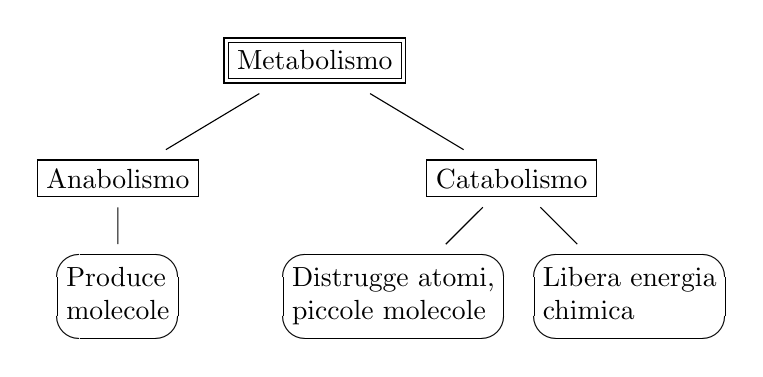
\begin{tikzpicture}[
        level 1/.style = {sibling distance = 5cm},
        level 2/.style = {sibling distance = 3cm},
    ]
    \node {\doublebox{Metabolismo}}
        child {
            node {\fbox{Anabolismo}}
            child {
                node {\ovalbox{\makecell[l]{Produce \\ molecole}}}
            }
        }
        child {
            node {\fbox{Catabolismo}}
            child {
                node {\ovalbox{\makecell[l]{Distrugge atomi, \\ piccole molecole}}}
            }
            child {
                node {\ovalbox{\makecell[l]{Libera energia \\ chimica}}}
            }
        };
    \end{tikzpicture}
\end{center}

\sexample{Catabolismo}{
    \begin{itemize}
        \item Urea (N)
        \item CO\({}_2\)
        \item H\({}_2\)O
    \end{itemize}
}

Il catabolismo produce ATP, mentre l'anabolismo serve per produrre materia.
\\
\textbf{Catalisi:}
Una reazione chimica necessita che i reagenti si incontrino e si scontrino in una determinata maniera.
Questa è una questione probabilsitica, e in genere molto rara.
Per diminuire la velocità di reazione si possono utilizzare dei catalizzatori.
L'esempio più semplice di catalizzatore è la temperatura, siccome l'aumento della temperatura
aumenta la velocità di movimento delle molecole e, per cui, porta un aumento della probabilità di collisione.
Tuttavia, l'aumento della temperatura nel corpo non è sempre auspicabile, e vengono utilizzati
quindi degli anzimi come catalizzatori.

\pagebreak

\begin{figure}[h]
    \centering
    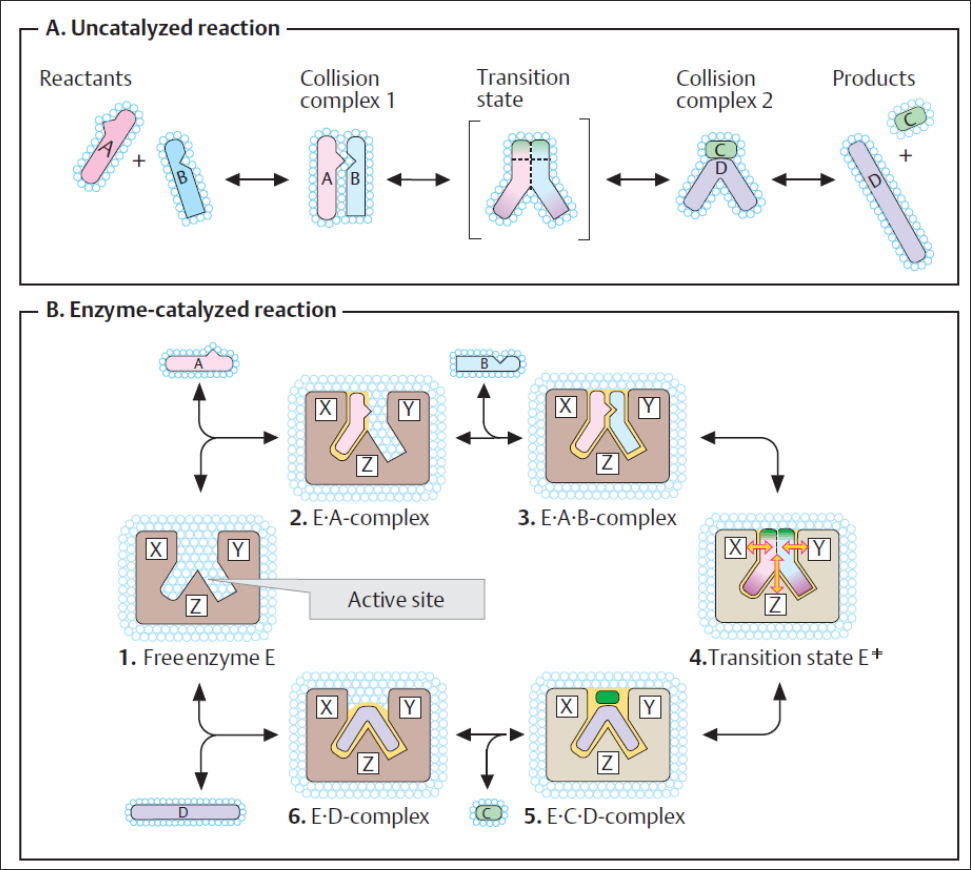
\includegraphics[width=0.95\textwidth]{./reactions_cat.png}
\end{figure}

Lo \textit{stato di transizione} è uno stato intermedio molto instabile.

Gli enzimi offrono un posto dove i reagenti possono adagiarsi in maniera da collidere nella maniera
corretta con gli altri reagenti.

L'energia necessaria per arrivare lo stato di transizione (con enzima) è nettamente
minore di quella per lo stato di transizione senza enzima.
Questo è dato dal fatto che senza enzima vi saranno molti urti fra reagenti ma senza reazione.
\[
    E_A = \textit{Energia di attivazione}
\]
Il posto dove vengono ospitati i reagenti nell'enzima si chiamano \textit{siti attivi}.

\pagebreak

\begin{figure}[ht]
    \centering
    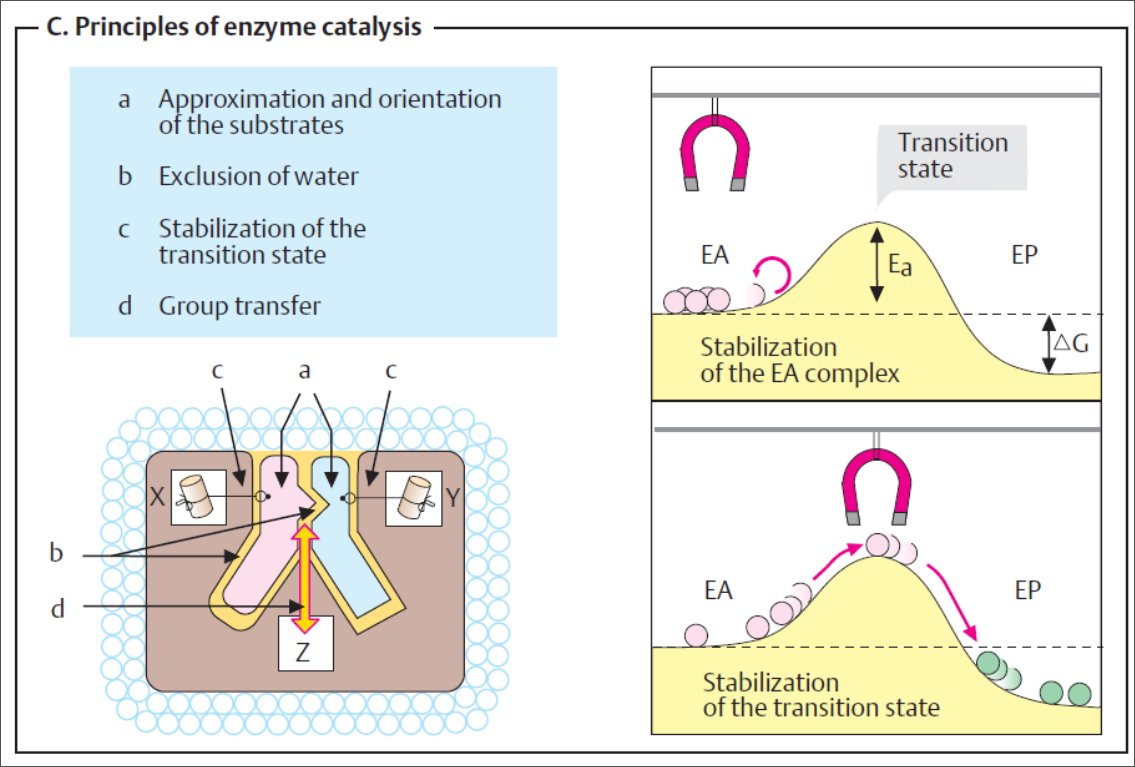
\includegraphics[width=0.95\textwidth]{./enzym_cat.png}
\end{figure}

L'enzima trascina i reagenti sullo stato di transizione.

\begin{figure}[ht!]
    \centering
    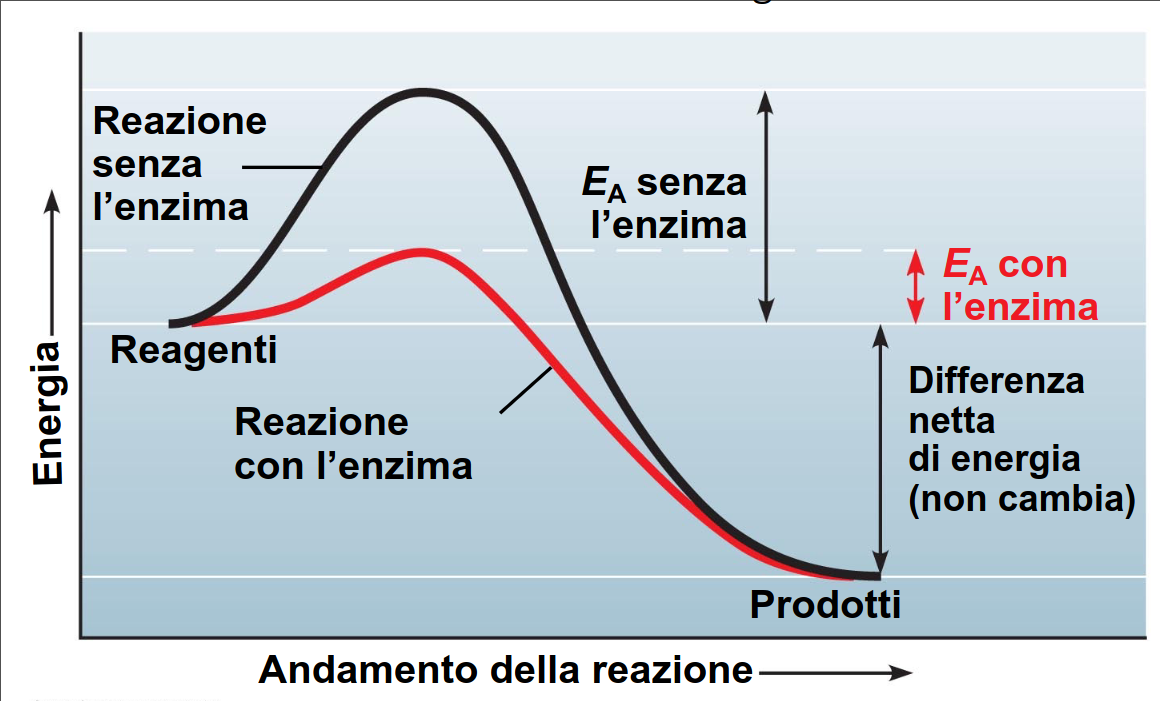
\includegraphics[width=0.85\textwidth]{./energy_reaction.png}
\end{figure}

\pagebreak

\subsubsection{Inibitori enzimatici}

\sdefinition{Inibitore enzimatico}{
    Con il termine \textit{inibitore enzimatico} si indica una molecola in grado di instaurare un legame chimico con un enzima, diminuendone così l'attività. 
}
È possibile che una molecola (inibitore), simile al reagente, occupi il 
posto nell'enzima dedicato al reagente. Questo blocca l'enzima e, per cui, la reazione chimica.
Gli inibitori vengono prodotti quando è necessario ridurre il numero reazioni chimiche
(Es. per feedback negativo, farmaco).

Gli inibitori possono essere due tipi:
\begin{itemize}
    \item \textbf{competitivo:} occupa il posto del reagente nello spazio ativo;
    \item \textbf{non competitivo:} deforma lo spazio attivo con un legame in un altra posizione.
\end{itemize}

Entrambi i tipi di inibitori possono essere \textit{reversibili} o \textit{irreversibili}.

\subsection{Respirazione cellulare}

\begin{figure}[ht!]
    \centering
    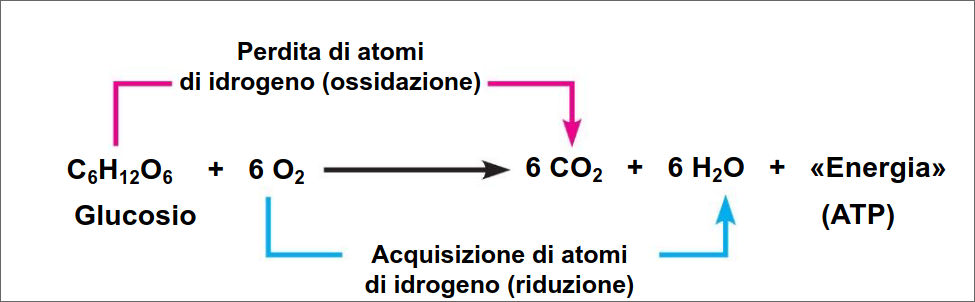
\includegraphics[width=0.85\textwidth]{./resp.png}
\end{figure}

La respirazione cellulare serve a spaccare i legami di una molecola grande
(tanti legami) e trasferirne l'energia chimica nell'ATP.
Gli atomi, H\({}_2\)O e CO\({}_2\) sono scarti. Gli elettroni servono nel processo per caricare l'ATP, per poi
essere scartati.

\sdefinition{Mitocrondrio}{
    Il \textit{mitocondrio} è un organello nella cellula dove avviene parte della respirazione cellulare.
}

Il mitocondrio è composto da due membrane, dividendosi in una parte interna ed esterna.

\sdefinition{Creatina}{
    La \textit{creatina} è una molecola che possiede un fosfato, il suo scopo è quello di aumentare la produzione di ADP.
}

Le cellule svolgono 3 tipi di lavoro: chimico, di trasporto e meccanico.
Il lavoro meccanico serve per far contrarre le fibre muscolari.

le 3 tappe della respirazione cellulare sono
\begin{enumerate}
    \item \textbf{Glicolisi}
    \item \textbf{Cliclo di Krebs} (all'interno del mitocondrio)
    \item \textbf{Fosforilazione ossidativa} (gradienti fra lo spazio intermembranan e lo spazio interno del mitocondrio)
\end{enumerate}

\sdefinition{Glicolisi}{
    La \textit{glicolisi} è una serie di reazioni chimiche che spaccano il glucosio in 2 \textit{piruvati} (\(C_3H_6O_3\)).
}

Questo procedimento produce (poco) ATP dallo spaccamento e libera elettroni.
Gli elettroni liberati vengono presi dall'NAHD (molecole di trasporto degli elettroni
che diventa FADH\({}_2\))
che le trasportano nella cellula.

Il piruvato entra nel ciclo di Krebs, dove esce il CO\({}_2\) per produrre l'Acetil-coenzima A.
L'Acetil-coenzima A viene spaccato, producendo una piccola quantità di ATP.
Vengono quindi spaccati tutti gli atomi, tenendo solo gli elettroni che vanno nel terzo processo.

Gli elettroni prodotti si avviano verso il mitocondrio. La cellula è interessata a portare
gli \(H^+\) contro grandiente verso lo spazio fra le 2 membrane.
Per trasportarli contro gradiente viene sfruttata l'energia degli elettroni che si muovono in saltando fra le proteine.

Gli elettroni vengono successivamente presi dall'ossigeno, che li usa per legare con gli \(H^+\) e formare
acqua.

\subsection{Fermantazione alcolica}

La fermantazione alcolica avviene in assenza di ossigeno e viene svolta prevalentmeente dagli lieviti (fungi unicellulari).
Lo lievito fa la fermentazione per vivere e svolgere le sue funzioni metaboliche.

Dopo aver prodotto l'energia, è necessario sbarazzarsi del piruvato protonato (acido piruvio),
viene quindi spaccato e scaricato nell'aria come Etanolo e CO\({}_2\).
% CO2 e Etanolo con REDOX scaricano NADH

\subsection{Fermantazione lattica}

La fermentazione lattica viene svolta da alcuni organismi come batteri.
Gli umani la svolgono dopo uno sforzo muscolare.
Il piruvato viene convertito in acido lattico (scarto), che viene poi smaltito dal fegato con ATP.

\pagebreak

\section{Anatomia e fisiologia della cellula}

Le prime forme di vita erano composte unicamente cellule precariote, ossia cellule 
senza nucleo. Non ci sono organelli o struttura interna, vi sono solo delle strutture
per produrre proteine.
Essi svolgono esclusivamente la glicolisi e non la respirazione cellulare.

Per costruire le proteine sono necessari i ribosomi.

\begin{figure}[th]
    \centering
    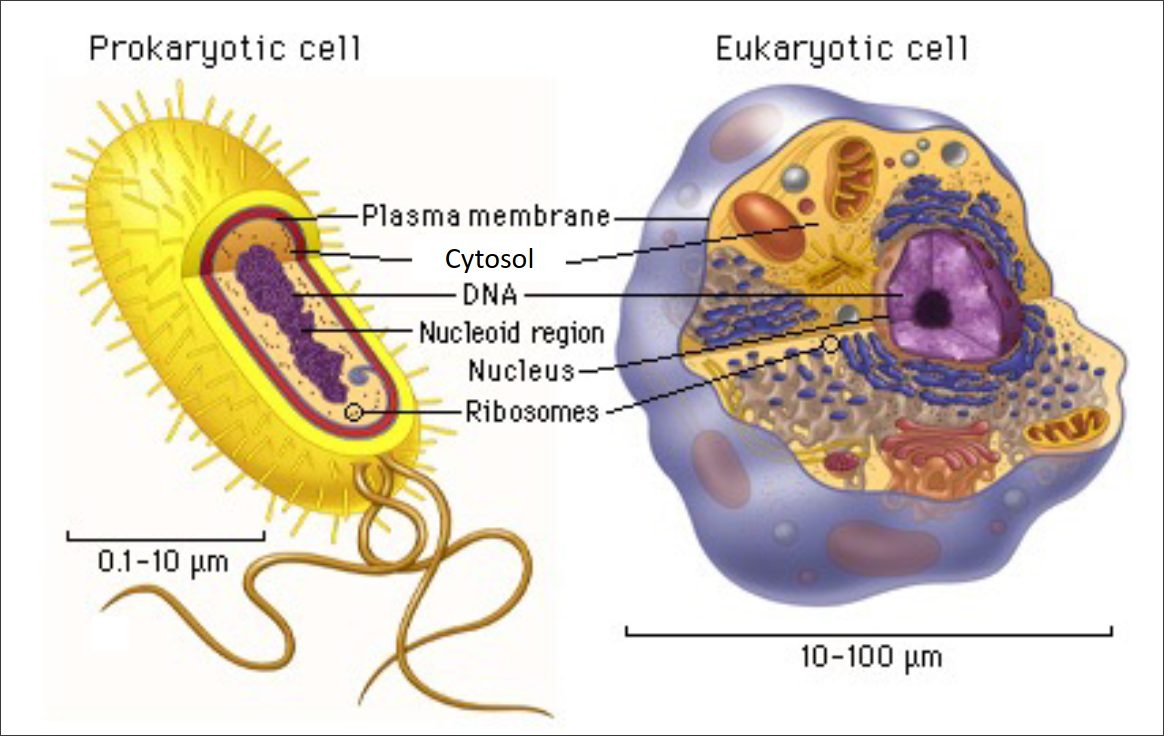
\includegraphics[width=0.75\textwidth]{./prok-euka.png}
\end{figure}

Con citosol si intende il solvente, mentre citoplasma l'intera soluzione.
\\
Gli spermatozoi sono delle cellule eucariote pieni di mitocondri.
Il DNA è protetto nel nucleo.

Se la cellula fosse troppo grande, avrebbe un rapporto area su volume troppo piccolo, e non riuscirebbe
a fare sufficientemente scsmbi sulla sua area superficiale.

\subsection{Gli organuli cellulari}

Le cellule sono le unità fondamentali degli esseri viventi, le più piccole unità biologiche che
mostrano tutte le caratteristiche della vita. Nonostante le loro piccole dimensioni, le cellule
animali e vegetali possono avere una diversa dotazione di organuli specializzati per i compiti
necessari alla loro sopravvivenza e al loro funzionamento. Ci concentreremo prima sugli
organuli presenti sia nelle cellule animali sia in quelle vegetali, e poi ci occuperemo di alcuni
organuli supplementari presenti solo nelle cellule vegetali.

Iniziamo dall'esterno della cellula. Tutte le cellule sono separate dall'ambiente esterno da
una membrana plasmatica. La \textbf{membrana plasmatica} è una parete sottile, a doppio strato,
che regola il traffico delle molecole in entrata e in uscita. Possiamo paragonarla alle pareti
di una casa. Le pareti hanno finestre e porte che possono essere aperte per far entrare e
uscire le cose dalla casa. Queste finestre e porte possono essere regolate - in altre parole
possiamo decidere quali aprire e quando aprirle. Allo stesso modo, la membrana plasmatica
possiede canali, formati da proteine, che regolano il passaggio di molecole specifiche in
entrata e in uscita dalla cellula. Si crea così una membrana semipermeabile tra l'interno
della cellula, il citoplasma, e l'ambiente esterno. Il termine “semipermeabile” si riferisce al
fatto che alcune sostanze possono attraversare la membrana, mentre altre non possono
farlo.

All'interno delle cellule animali e vegetali, uno degli organuli più evidenti è il nucleo. Il nucleo
contiene il DNA, l'informazione genetica che controlla l'attività della cellula. Possiamo
pensare al nucleo come al “cervello” della cellula. Il nucleo è circondato da una membrana
chiamata \textbf{involucro nucleare}. Come la membrana plasmatica, questa struttura serve a
regolare il traffico delle molecole. In questo caso, l'involucro nucleare controlla il flusso delle
molecole tra il nucleo e il resto della cellula.

Molti dei materiali che escono dal nucleo vengono trasportati attraverso il sistema di
membrane endocellulari. Il \textbf{sistema di membrane endocellulari} è una rete di organuli che
produce e distribuisce i prodotti cellulari. Questi organuli comprendono il reticolo
endoplasmatico, l'apparato di Golgi e i lisosomi. Vediamo ora qual è la funzione specifica di
ognuno di questi organuli.
% lisosom

Il \textbf{reticolo endoplasmatico}, abbreviato con la sigla RE, è il principale centro di produzione
della cellula. In una cellula esistono due tipi di RE: il RE ruvido e il RE liscio. Il RE ruvido è
provvisto di ribosomi sulla superficie esterna, che al microscopio lo fanno appunto apparire
“ruvido”.

I \textbf{ribosomi} sono delle strutture (non organelli) responsabili della produzione delle proteine. Se il reticolo
endoplasmatico è la “fabbrica” della cellula, i ribosomi sono i singoli macchinari che ne
realizzano i prodotti. Il RE liscio si chiama così perché è privo di ribosomi. La sua funzione
principale è la costruzione dei lipidi.

Spesso, i materiali prodotti nel RE passano poi all'\textbf{apparato di Golgi}. L'apparato di Golgi è
come un centro di perfezionamento e impacchettamento. Al suo interno, le proteine
vengono modificate, etichettate e inviate alle aree di destinazione della cellula. Per molti
versi, l'apparato di Golgi corrisponde all'ufficio postale della cellula, che etichetta le proteine
e le indirizza alla destinazione corretta.

L'ultimo organulo del sistema di membrane endocellulari di cui ci occupiamo è il \textbf{lisosoma},
presente solo nelle cellule animali. Il lisosoma è un organulo costituito da enzimi digestivi
racchiusi da una membrana. La sua funzione principale è la demolizione delle sostanze,
come i prodotti di rifiuto o gli organuli vecchi. Le molecole risultanti vengono spesso riciclate
e quindi usate per produrre nuovi composti in altri punti della cellula. Possiamo pensare al
lisosoma come al “tritarifiuti” della cellula.

I \textbf{mitocondri} sono i principali organuli cellulari per la produzione di energia. Sono il centro
primario in cui si svolge la respirazione cellulare, in cui l'energia degli zuccheri e delle altre
molecole nutritive viene trasformata in ATP. L'ATP è una piccola molecola usata dalle cellule
per alimentare la maggior parte del lavoro. Le cellule che consumano molta energia, come
quelle del cervello o dei muscoli, hanno molti mitocondri, che producono molta ATP.

L'ultima struttura di cui ci occupiamo, comune alle cellule animali e vegetali, è il
\textbf{citoscheletro}. Il citoscheletro è la struttura di sostegno della cellula. Come dice il suo nome,
possiamo immaginarlo come uno scheletro o un'impalcatura che dà forma alla cellula e
fornisce un punto di attacco per gli altri organuli così da non lasciarli semplicemente fluttuare
per la cellula. Il citoscheletro viene utilizzato anche come “autostrada” grazie a particolari
proteine che vi trasportano le molecole, come camion su una strada.

Tutti gli organuli che abbiamo descritto finora, fatta eccezione per i lisosomi, sono presenti
sia nelle cellule vegetali sia in quelle animali. Descriveremo ora altri tre organuli/strutture
esclusivi delle cellule vegetali: la parete cellulare, il vacuolo centrale e i cloroplasti.

La \textbf{parete cellulare} è uno strato rigido protettivo situato all'esterno della membrana
plasmatica. Nelle piante, la parete cellulare è formata da una sostanza chiamata cellulosa.
Avete mai strappato un filamento da un gambo di sedano? Quel filamento è formato in gran
parte dalla cellulosa delle pareti cellulari.

All'interno delle cellule vegetali, il vacuolo centrale è spesso l'organulo più grande. Il
\textbf{vacuolo centrale} ha una struttura a sacco delimitata da una membrana che serve come
magazzino e contribuisce a regolare la quantità di acqua nella cellula.

L'altro organulo esclusivo delle piante è il \textbf{cloroplasto}, un organulo per la produzione di
energia, presente solo nelle cellule vegetali. Quale organulo per la produzione di energia
abbiamo già descritto? Giusto, il mitocondrio. I mitocondri sono specializzati nella
produzione di ATP a partire dagli zuccheri. I cloroplasti, invece, sono specializzati
nell'utilizzare l'energia della luce solare per produrre gli zuccheri. Riuscite a vedere il
collegamento? I cloroplasti sfruttano l'energia luminosa per produrre zuccheri, e i mitocondri
utilizzano gli zuccheri per produrre ATP. Le cellule vegetali hanno sia i cloroplasti sia i
mitocondri: i cloroplasti per produrre gli zuccheri a partire dall'energia della luce solare, e i
mitocondri che producono ATP a partire da questi zuccheri. Le cellule animali, tuttavia,
hanno soltanto mitocondri, il che significa che non possono prodursi da sole gli zuccheri. Gli
animali devono quindi mangiare piante o altri animali per ottenere gli zuccheri, necessari ai
mitocondri per produrre l'ATP.

% TODO feedback negativo2

% TODO Pompa sodio-potassio porta fuori sodio e dento potassio (crea un gradiente), esempio di trasporto attivo primario

\pagebreak

\subsection{Produzione di proteine}

% microscopio classico
% " meccanico (con elettroni)
% " fluorescente (che lega con le molecole)

\begin{figure}[th]
    \centering
    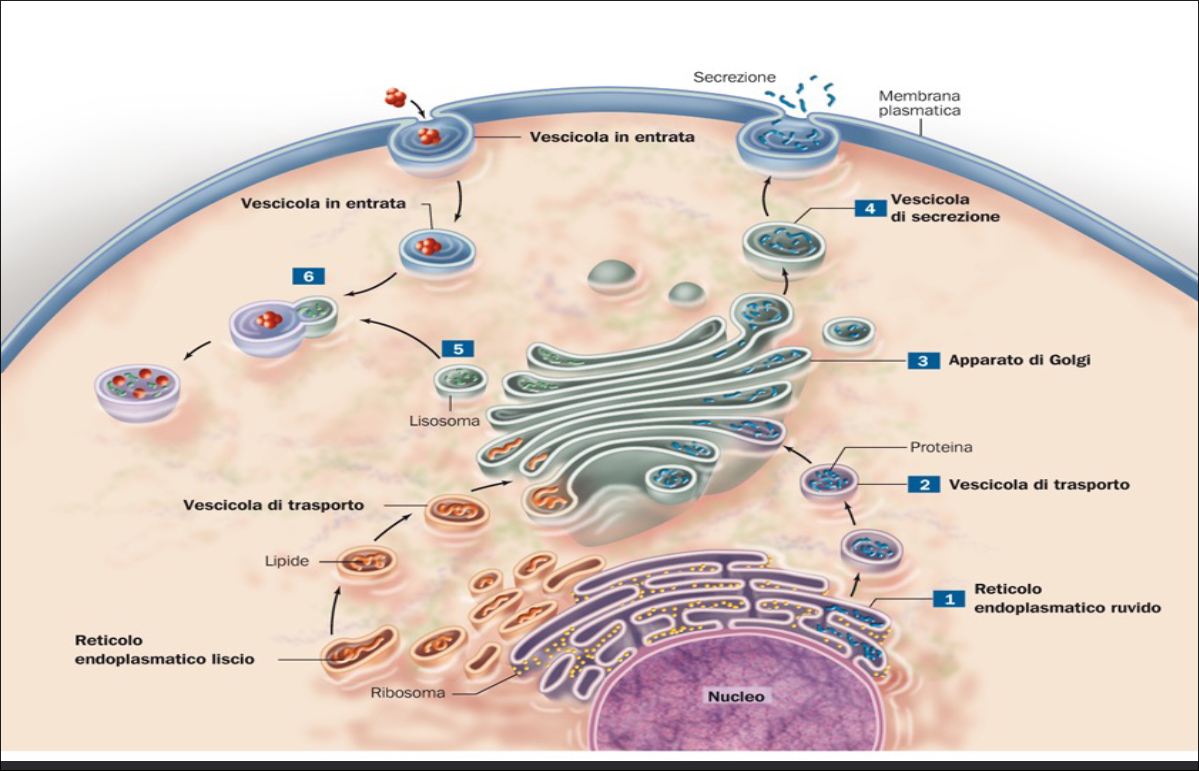
\includegraphics[width=0.75\textwidth]{./prod_cellula.png}
\end{figure}

Le proteine vengono prodotte con le informazioni (nel nucleo).
Quando l'informazione è necessaria ne viene fatta una copia nel nucleo.
Questa informazione viene letta dal ribosoma.
Il ribosoma (struttura - un ammasso di proteine) legge l'mRNA,
dove c'è scritto dove mettere gli amminoacidi per costruire le proteine.

\begin{figure}[th]
    \centering
    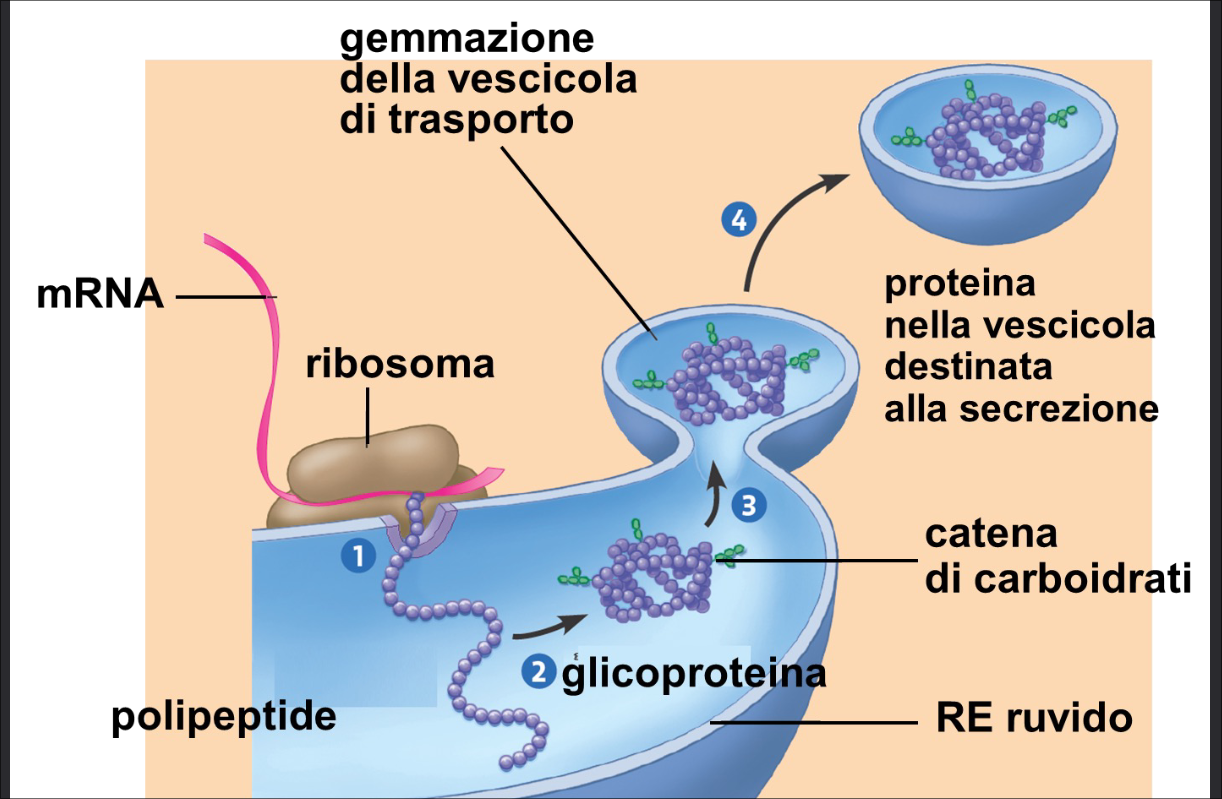
\includegraphics[width=0.75\textwidth]{./prod_cellula2.png}
\end{figure}

% che sia una glicoproteina è un esempio
Il contorno blu (reticolo endoplasmatico) è come una membrana cellualre. Il ribosoma si appoggia e inserisce la proteina.
La vescicola del reticolo si stacca e si unisce all'apparato di Goigi, dove le proteine
vengono completate e indirizzate.
La proteina se ne va nuovamente con una vescicola, la vescicola si fonde alla membrana (diventa parte della membrana)
e per esocitosi ne uscirà il contenuto.

Nel reticolo endoplasmatico liscio vengono creativi dei fosfolipidi.
Siccome le vescicole accorciano il reticolo, questi fosfolipidi servono a refillarlo.

Gli enzimi dei isosomi vengono costruiti dai ribosomi nel reticolo endoplasmatico ruvido.

\pagebreak

\begin{figure}[th]
    \centering
    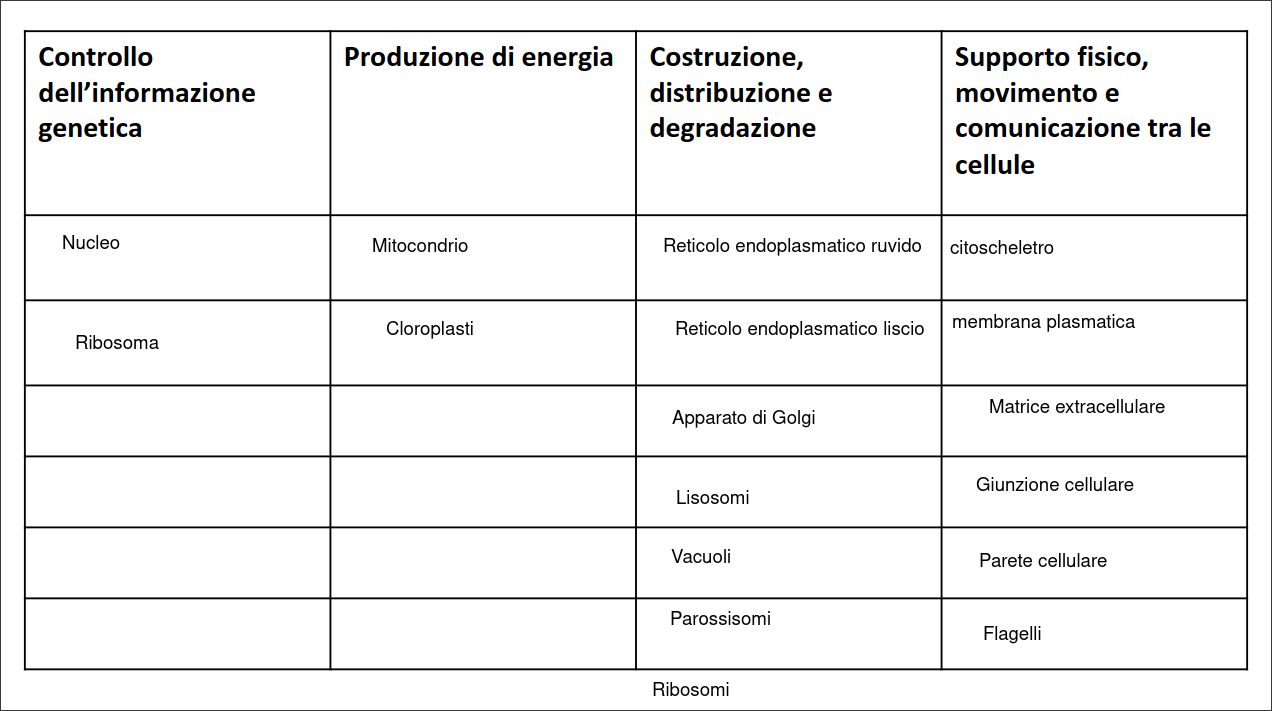
\includegraphics[width=\textwidth]{./strutture.png}
\end{figure}

\pagebreak

\subsection{Osmosi}

Le particelle nel soluto si spostano fra le membrane semi-permeabili secondo il gradiente
di concentrazione. Quando non è possibile raggiungere un equilibrio spostando il soluto,
l'equilibrio si può raggiunto per spostamento del solvente (acqua) piuttosto che il soluto.

\sdefinition{Osmosi}{
    Per \textit{osmosi} si intede il passaggio spontaneo dell'acqua (solvente) attraverso una membrana semi-permeabile
    per raggiungere un equilibrio elettrochimico.
}

\sdefinition{Osmoregolazione}{
    Per \textit{osmoregolazione} si intende l'intervento ativo che fa l'organismo per evitare di subire le conseguenze del movimento spontaneo dell'acqua.
}

\begin{figure}[th]
    \centering
    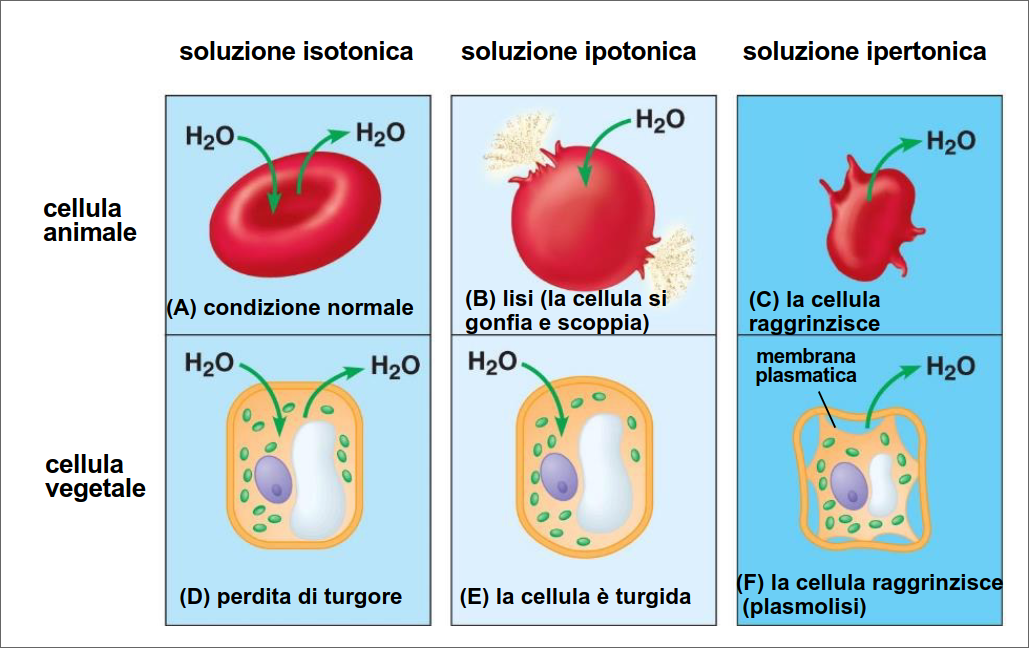
\includegraphics[width=0.75\textwidth]{./equilibrio_idrico.png}
\end{figure}

La cellula vegetale non scoppia perché ha la parete per contenere.

\pagebreak

\section{Biologia Umana}

\subsection{Sistema digerente e nutrizione}

La trasformazione del cibo avviene in quattro fasi distinte.
\begin{enumerate}
    \item \textbf{ingestione;}
    \item \textbf{digestione:} demolizione del cibo. Viene convertito in molecole sempre più piccole per essere
    assorbite dal corpo. La maggior parte delle molecole che costituiscono il cibo sono
    biomolecole e sono grandi;
    \item \textbf{assorbimento:} avviene grazie alle cellule che rivestono il tubo digerente.
    Le molecole vengono scomposte in piccoli pezzi come aminoacidi o piccoli zuccheri;
    \item \textbf{eliminazione:} scarti che vengono
    espulsi dal tubo digerente.
\end{enumerate}

Tutto parte dal tubo digerente e delle ghiandole a esso associate:
Ghiandole salivali, pancreas e fegato. I denti e la lingua sono organi
della cavità orale e sono annessi al sistema digerente.
Il cibo introdotto dalla bocca e masticato dai denti viene spinto dalla
lingua alla faringe.

\sdefinition{Peristalsi}{
    La \textit{peristalsi} è un processo in cui ci sono delle onde di
    contrazione e rilassamento dei muscoli lisci presenti nella
    parete del tubo digerente.
}

Dopo essere stato deglutito viene sospinto dal
processo di peristalsi.
\\
In una decina di secondi il cibo passa dall'esofago allo stomaco. Due
valvole muscolari, chiamate sfinteri, regolano il passaggio del cibo.

\begin{enumerate}
    \item Il cardias regola il passaggio dall'esofago allo stomaco
    \item Il piloro regola il passaggio dallo stomaco all'intestino tenue
    Il piloro permette al cibo di rimanere chiuso nello stomaco dalle.
    2 alle 6 ore, così da permettere ai succhi gastrici e agli enzimi
    di cominciare la digestione
\end{enumerate}

La fase finale della digestione e l'assorbimento avvengono
nell'intestino tenue nell'arco di 5-6 ore. Le sostanze non digerite
continuano nell'intestino crasso, l'acqua viene riassorbita e il restante
si tramuta in feci che verranno poi espulse. Per questo processo ci
vogliono dalle 12 alle 24 ore.

\subsubsection{Bocca}

La secrezione che si trova all'interno della bocca è la saliva e l'enzima
presente è l'\textbf{amilasi salivare}.
Sono presenti altre sostanze come la mucina (il muco).
L'amilasi salivare scompone l'amido in maltosio e destrine. (oligosaccaridi ?)

\pagebreak

\begin{figure}[th]
    \centering
    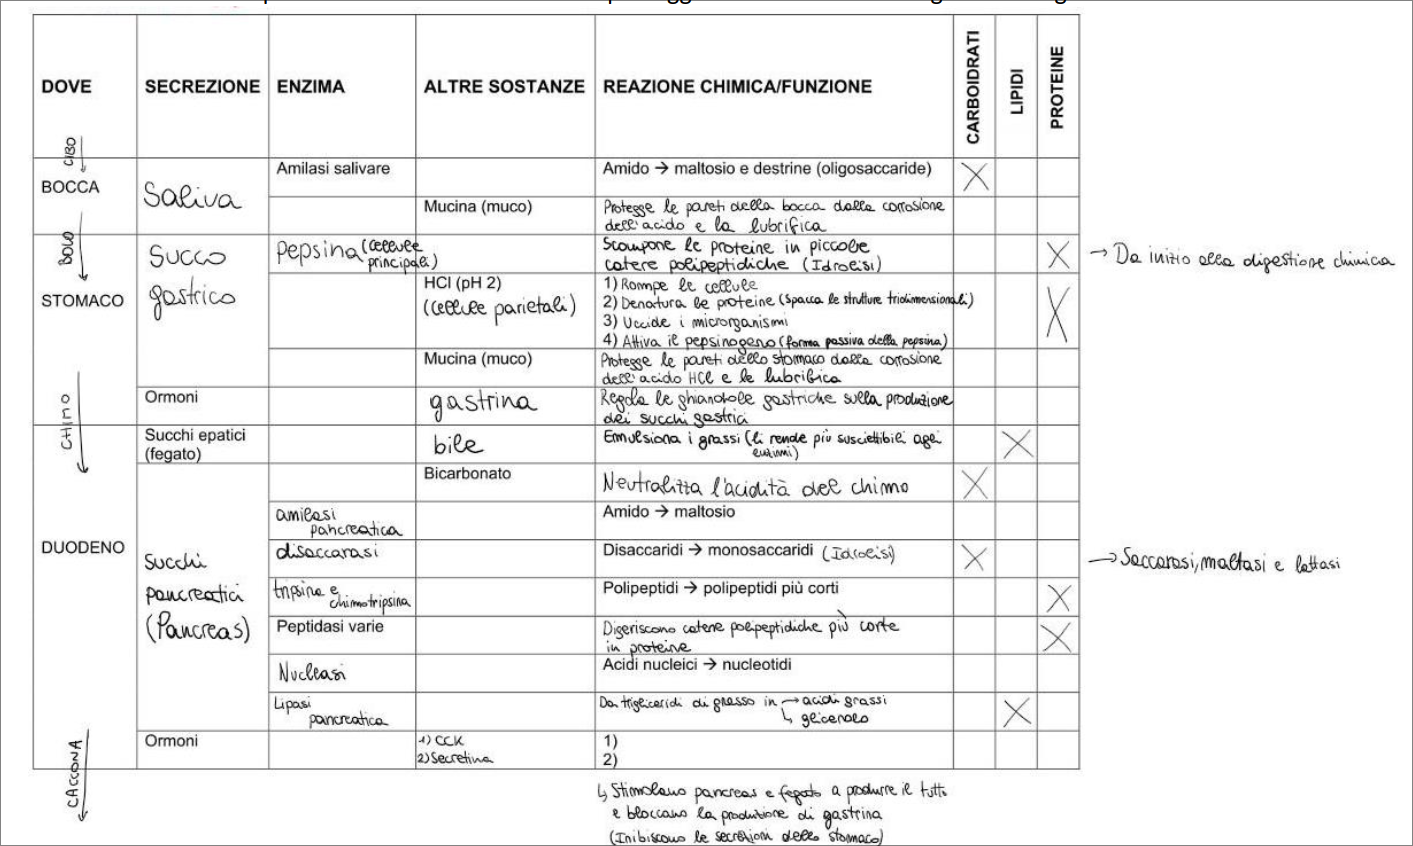
\includegraphics[width=\textwidth]{./tabella.png}
\end{figure}

\sexercise{Spiegare in modo dettagliato come viene attivata e mantenuta la produzione di succhi gastrici a
livello dello stomaco}{
    La primissima attivazione della digestione parte da impulsi nervosi che scaturiscono dai sensi
    (es. odore o vista etc.).
    Subito dopo la masticazione stimola principalmente la produzione.
    Una volta giunti nello stomaco le cellule della parate dello stomaco vengono stimolate e producono la gastrina.
    La gastrina a sua volta stimolerà il resto della digestione.
}

\sexercise{Spiegare come fa lo stomaco a sapere che deve smettere di produrre succhi gastrici}{
    La gastrina viene continuamente prodotta ed essa stimola la produzione di succhi gastrici.
    Inoltre, vi è un meccanismo di feedback positivo che stimola la produzione di succhi gastrici.
    Più pepsina c'è, più si attiva il pepsinogeno, per cui in breve tempo la concentrazione di pepsina aumenta esponenzialmente.
}

\sexercise{Spiegare come fa lo stomaco a sapere che deve smettere di produrre succhi gastrici}{
    Il chimo acido esce dallo stomaco ed entra nel duodeno.
    Quando non c'è il chimo lo stomaco continua a produrre succhi gastrini,
    ma vi è un sistema di feedback negativo che ne blocca la produzione.
    Questo feedback negativo è attivato dal fatto che l'acidità dello stomaco aumenta.
    Inoltre, il chimo viene percepito dalle cellule della parete del duodeno, le quali iniziano a produrre
    due ormoni (che vanno nel sangue come tutti gli ormoni), ossia il CCK (colecistochemica) e la secretina.
    Gli ormoni raggiungono il pancreas ed il fegato.
    Il fegato rilascia la bile che viene depositata nella cistifellea.
    Il CCK stimola la cistifellea a rilasciare la bile.
    Il CCK e la secretina bloccano la produzione di gastrina.
}

% sono nella 3
%\sexercise{Spiegare cosa è il CCK, dove viene rilasciato e quando}{
%\sexercise{Elencare i passaggi che portano alla produzione di succhi pancreatici. Partire dall'arrivo del chimo}{

\pagebreak

\begin{figure}[th]
    \centering
    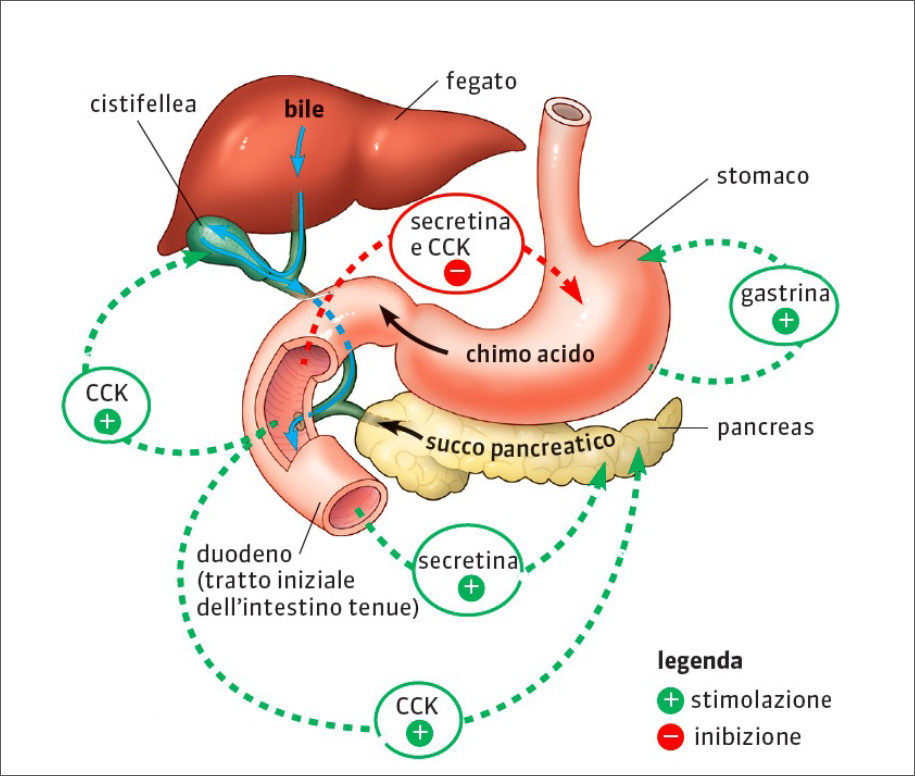
\includegraphics[width=0.5\textwidth]{./digestione.png}
\end{figure}

Nell'intestino tenue vengono assorbiti:

\begin{itemize}
   \item Monosaccaridi
   \item Amminoacidi
   \item Acidi grassi e glicerolo
   \item Nucleotidi
   \item Vitamine
   \item Acqua
   \item Sali minerali
\end{itemize}

\begin{figure}[th]
    \centering
    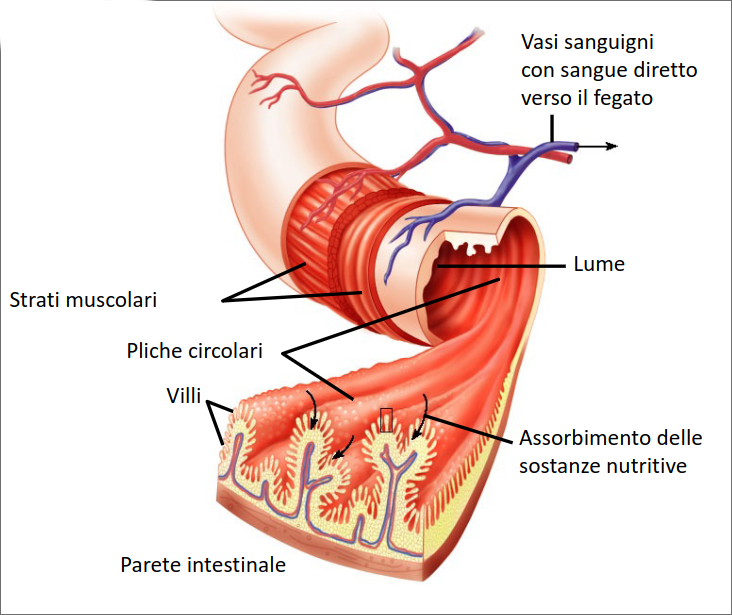
\includegraphics[width=0.75\textwidth]{./intestino.png}
\end{figure}

\pagebreak

\begin{figure}[th]
    \centering
    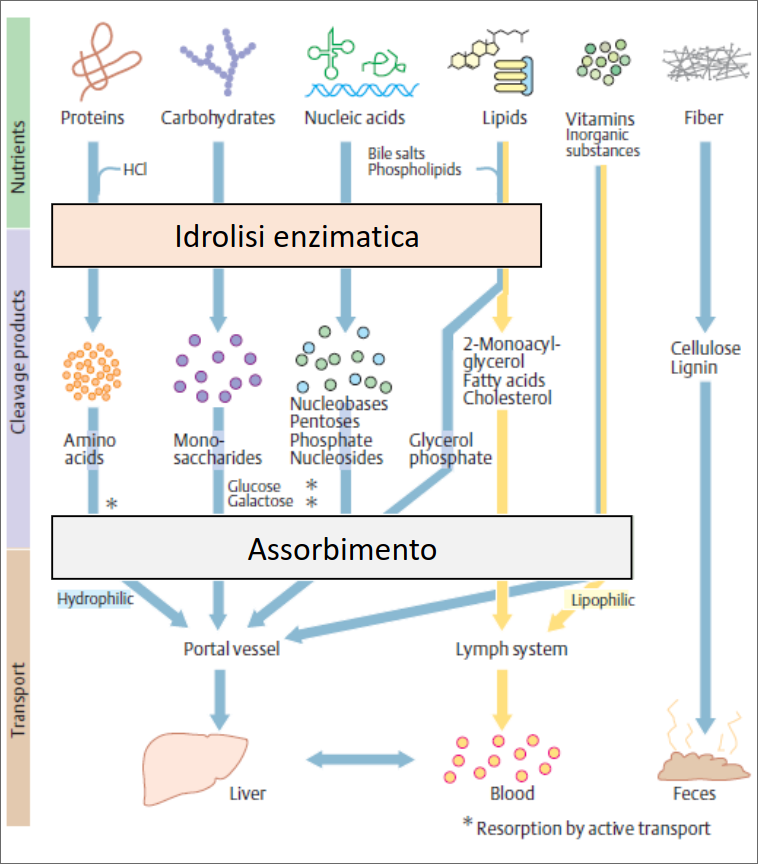
\includegraphics[width=\textwidth]{./assorbimento.png}
\end{figure}

Le fibre non hanno un vero valore nutrizionale ma permettono un miglior assorbimento delle sostanze fibrose.

\pagebreak

\begin{figure}[th]
    \centering
    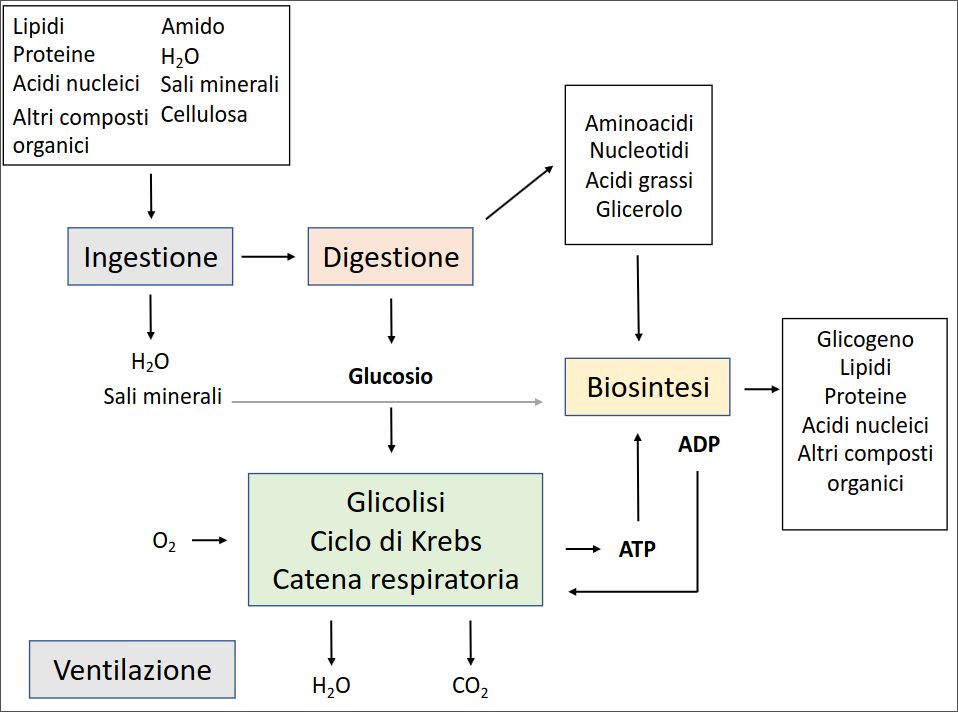
\includegraphics[width=\textwidth]{./nutrizione.png}
\end{figure}

\sexercise{Da dove arrivano gli amminoacidi che vengono
assorbiti dall'intestino? Descrivere il loro percorso.}{
    Vengono principalmente ingeriti dopo essere masticati e lubrificati, dopodiché passano attraverso
    l'esofago ed entrano nello stomaco. Una volta che il bolo si trova all'interno dello stomaco,
    viene scomposto dalla pepsina e dai succhi gastrini (HCL), la cui produzione viene stimolata dalla gastrina.
    Il bolo diventa quindi chimo acido, il quale entrando nel duodeno ne stimola le pareti producendo
    CCK e secretina. La secretina stimola il pancreas a rilasciare una soluzione di bicarbonato di sodio
    nel duodeno che neutralizza l'acidi del chimo.
    Il CCK, invece, stimola il rilascio dal fegato dei succhi epatici e del pancreas i succhi pancreatici.
    Dopo aver attraversato il duodeno il prodotto (chilo, chimo neutralizzato) attraversa il digiuno e l'ileo dove
    viene completata l'assunzione delle sostanze nutritive.
    Gli amminoacidi (proteine idrolizzate in precedenza nel duodeno grazie agli enzimi) vengono assorbiti dalla parete intestinale (grazie ai vili e ai microvilli).
}

\sexercise{Cosa succede agli amminoacidi una volta assorbiti a
livello intestinale? Per rispondere alla domanda
considerare i seguenti punti:}{
    \begin{enumerate}
        \item L'urea è un prodotto del metabolismo delle proteine che
            viene eliminato attraverso le urine
        \item Nel fegato gli amminoacidi possono essere trasformati in
        zuccheri, grassi o precursori dell'ATP
        \item Gli enzimi digestivi (come per esempio la pepsina o la
        lipasi) sono delle proteine.
    \end{enumerate}

    XXXXXXXXXXX % chiedi a Dijana :)
    % una volta finiti nel sangue vengono utilizzati per l'anabolismo o eliminati se in eccesso.
}

Otto amminoacidi su 20 sono essenziali, e per cui devono per forza essere assorbiti dall'alimentazione
siccome non possono essere prodotti. 
Se la cellula non necesita di amminoacidi, essi vanno principalmente al fegato, il quale si occupa
di sfruttare questa materia organica in eccesso, ossia convertendola in glucosio o lipidi.

\begin{center}
\begin{figure}[th]
    \centering
    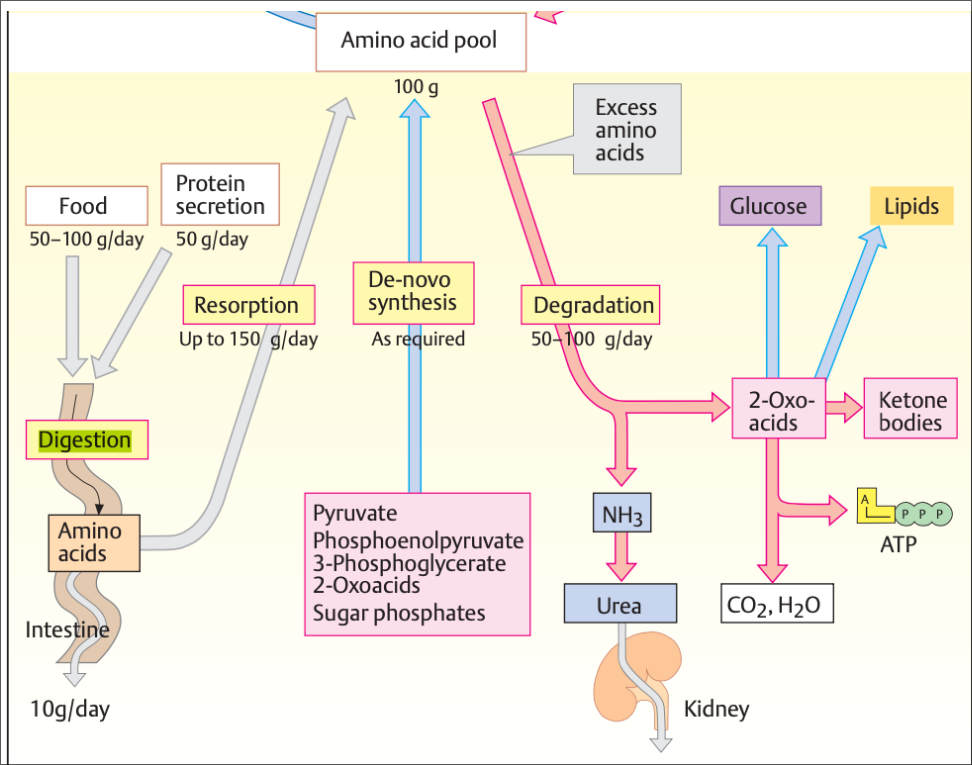
\includegraphics[width=0.6\textwidth]{./ciclo_amminoacidi.png}
\end{figure}
\end{center}

\begin{center}
\begin{figure}[th]
    \centering
    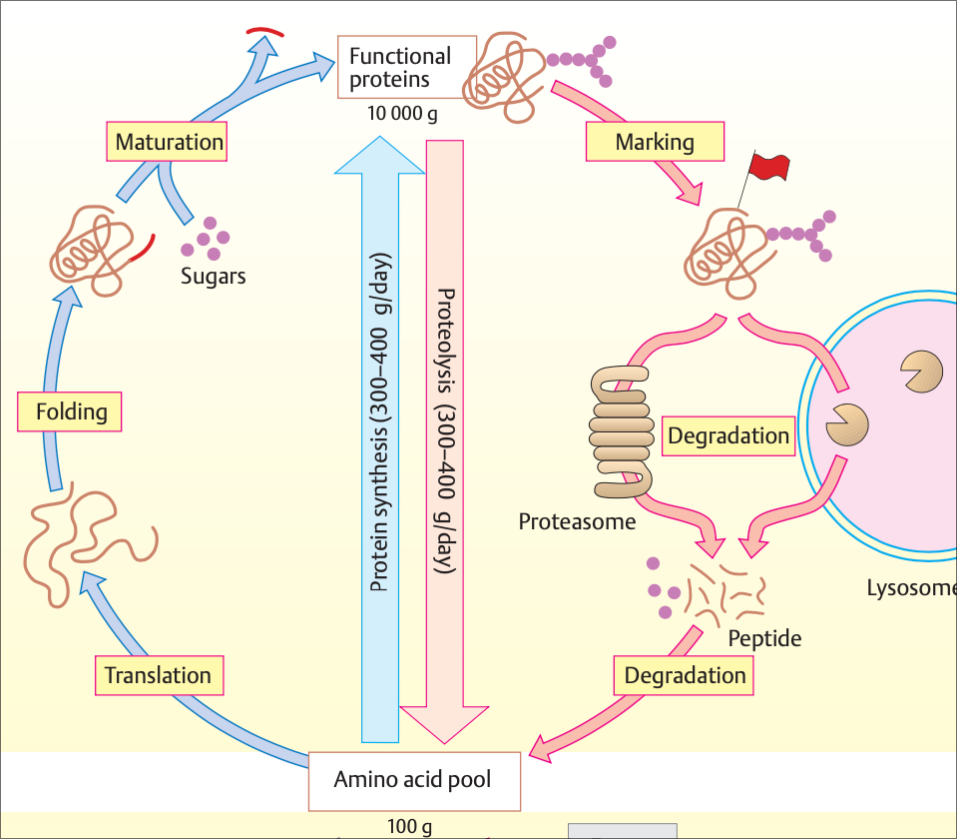
\includegraphics[width=0.6\textwidth]{./protein_metabolism.png}
\end{figure}
\end{center}

\pagebreak

\begin{center}
\begin{figure}[th]
    \centering
    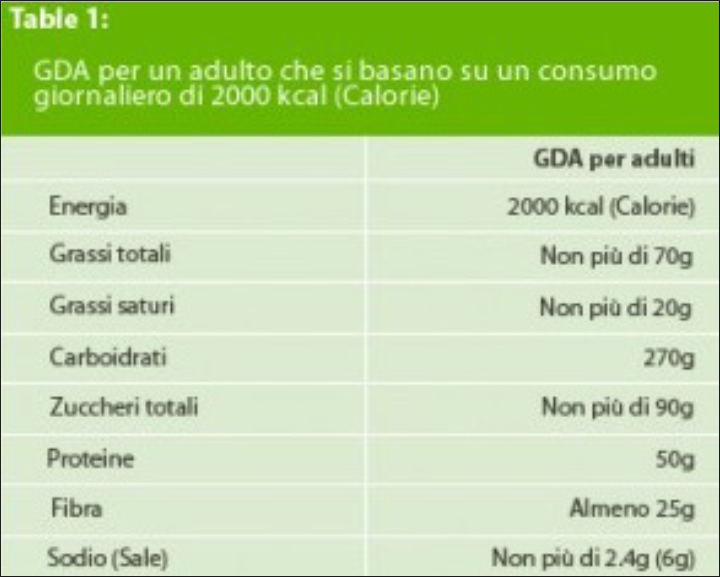
\includegraphics[width=0.75\textwidth]{./daily_intake.png}
\end{figure}
\end{center}

Il corpo ha bisogno anche di determinati tipi di elementi per svolgere determinate tipi di funzioni.

\sdefinition{Metabolismo basale}{
    Con \textit{metabolismo basale} si intende la quantità di energia impiegata in condizioni di neutralità termica.
}

\pagebreak

\subsection{Apparato cardiocircolatorio}

\subsubsection{Sistema circolatorio}

\sdefinition{Sistema circolatorio}{
    Il \textit{sistema circolatorio} umano è un sistema chiuso
    che trasporta il sangue, contenente varie sostanti, in giro nell'organismo pluricellulare.
}

Nel caso di organismi primitivi, per cui non abbastanza complessi da necessitare un sistema circolatorio,
non è necessario o possibile averne uno.
L'organismo semplice è a contatto con l'ambiente e scambi energia sul momento.

L'apparato circolatorio svolge i seguenti ruoli:
\begin{itemize}
    \item \textbf{Trasporto:} 
    \begin{itemize}
        \item di \textit{gas} (O\({}_2\), CO\({}_2\)) trasporto passivo, diffusione semplice, polmoni \(\iff\) sangue;
        \item di \textit{metaboliti} (molecole del metabolismo), fra \(\iff\) (muscoli, reni, intestino dove vengono assorbiti, fegato dove vengono scartati);
        \item di \textit{ormoni}, cellule o ghiandole endocrine, servono come segnale e raggiungono il proprio bersaglio. % es cellula G
    \end{itemize}
    \item \textbf{Omeostasi:} mantenere alcuni parametri costanti (omeostasi), quali
        \begin{itemize}
            \item \textit{temperatura} (termoregolazione);
            \item \textit{equilibrio idrico} (idroregolazione), modificato la concentrazione dei soluti del sangue influenzando l'osmosi;
            \item il \textit{pH}, grazie all'aggiunta di sostanze acide o basiche.
        \end{itemize}
    \item \textbf{Difesa:} contiene alcune sostanze per la difesa del corpo umano, quali:
        \begin{itemize}
            \item \textit{globuli bianchi}, per distruggere organismi patogeni;
            \item \textit{anticorpi}, proteine per immobilizzare i patogeni;
            \item \textit{agenti coagulanti} (es. fibrina e piastrina), per riparare le ferite.
        \end{itemize}
\end{itemize}

Il sistema cardiocircolatorio umano è composto nella seguente maniera:
\begin{itemize}
    \item \textbf{sangue:} fluido circolante (plasma + elementi cellulari);
    \item \textbf{sistema di vasi:} arterie, arterioli, vene, venule e capillari;
        Le vene riportano il sangue al cuore mentre le arterie introducono quello ossigenato.
        I capillari sono dei tubi molto piccoli nei tessuti dove avviene lo scambio fra sangue e tessuto;
    \item \textbf{cuore:} pompa, motore che permette circolazione del sangue.
        \begin{itemize}
            \item diviso in due parti separati, ciascuna con 2 cavità, un'entrata e un'uscita;
            \item circolazione sistemica e polmonare separate;
            \item cuore più performance (grazie alla separazione in 4);
            \item soddisfa elevate necessità metaboliche.
        \end{itemize}
\end{itemize}

\pagebreak

Il sangue è composta da una parte cellulare (45\% volume) ed una plasmatica.
\begin{center}
\begin{figure}[th]
    \centering
    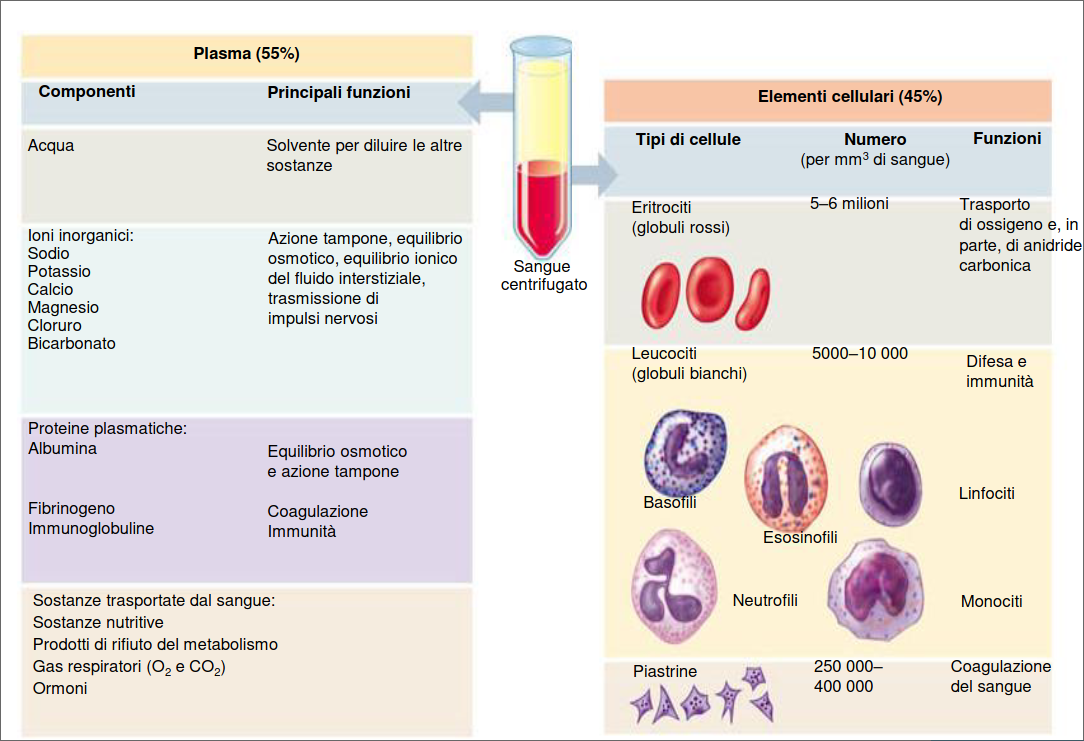
\includegraphics[width=0.9\textwidth]{./blood_composition.png}
\end{figure}
\end{center}

\subsubsection{Evoluzioni nei vertebrati}

\begin{center}
\begin{figure}[th]
    \centering
    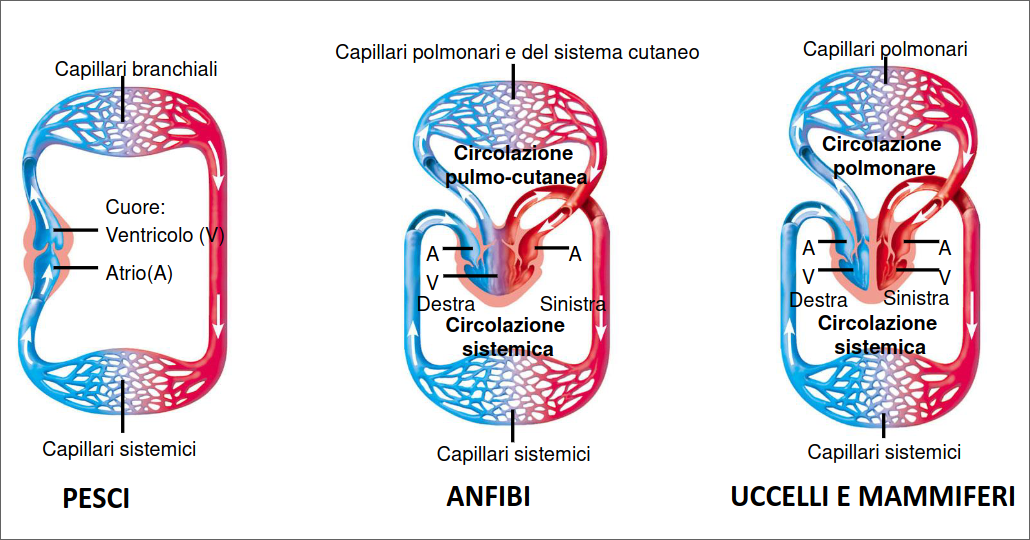
\includegraphics[width=0.75\textwidth]{./circulation_evolution.png}
\end{figure}
\end{center}

\sexercise{Come mai i vertebrati terrestri una circolazione unica non è sufficiente?}{
    Gli uccelli e mammiferi possiede un ventricolo in più rispetto agli anfibi.
    Il problema degli anfibi è che il sangue viene mischiato in un unico punto, rendendo un'efficienza minore (contiene sempre un po' di CO2).
    I pesci necessitano di una sola circolazione: il sangue decellera nei capillari (perché sì passa da un tubo grande a tanti piccoli, aumenta l'attrito),
    dai capillare alle branchi il sangue riparte e va ovunque nel pesce. Dai capillari sistemici esso torna al cuore.
    Siccome il sangue è fermo, non vi è una spinta per portarlo avanti.
    Questa spinta viene dalla compressione del tubo, ossia i muscoli che permettono al pesce di nuotare
    spingono il sangue. Ne consegue che i pesci non possono stare fermi.
    Per i pesci è facile nuotare perché la gravità non è così forte, data la presenza della forza di Asrchimede.
    Negli anfibi, il cuore contraendosi spinge sia la circolazione polmonare che sistemica.

}

\sexercise{Circolazione sistemica e polmonare}{
    La circolazione polmonare prevede la circolazione del sangue fra il cuore, i polmoni e viceversa,
    mentre la circolazione sistemica prevede la circolazione del sangue fra il cuore e il resto del corpo e viceversa.
}

\subsubsection{Anatomia del cuore}

\begin{center}
\begin{figure}[th]
    \centering
    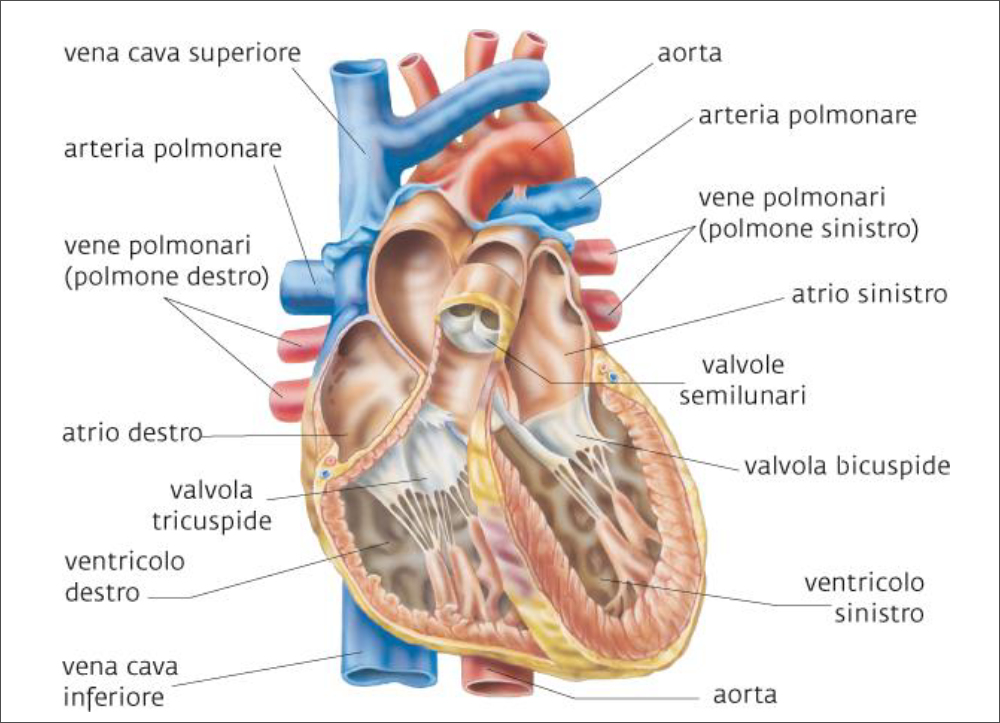
\includegraphics[width=0.9\textwidth]{./heart.png}
\end{figure}
\end{center}

Il ventricolo sinistro è più grosso perché spinge il sangue ossigenato in tutto il corpo,
mentre il ventricolo destro spinge solamente verso il polmone, il quale, è relativamente vicino.

Le 4 camere di chiamano atri e ventricoli.
Dall'atrio al ventricolo abbiamo una valcola che si chiude quando il sangue fluisce
per evitare un reflusso (valcole atrioventricolari destra e sinistra).

Dal ventricolo sinistro arriviamo all'aorta, ossia l'arteria principale.
Una volta giunto ai tessuti, il sangue ritorna mediante una vena al cuore.
Le vene che entrano a destra sono 2 (una dalla parte inferiore del corpo, e una dalla parte superiore).
Queste due vene si chiamano \textit{vena cava inferiore} e \textit{vena cava superiore}.
La vena che porta il sangue ossigenato al cuore si chiama vena polmonare, ed entra nell'atrio sinistro.

%%%%%%%%%%%%%%%%%%%%%%%%%%% schemino circolazione nei mammiferi

I nutrienti vengono caricati nel sangue, per cui tutta la circolazione polmonare e sistemica
è anche ricca di nutrienti. Nella vena cava inferiore vi è molto nutrimento
(come tutte le vene che vi ci uniscono), mentre nella vena cava superiore ve ne sono pochi.

% schema valcole valcole semilunari e atrioventricolari

\subsubsection{Struttura dei vasi sanguigni}

I capillari hanno pareti molto sottili, costituite da un singolo strato di cellule epiletali.
Arterie, arteriole, vene e venule hanno pareti più spesse, rivestite da un epitelio e rinforzate da uno strato di tessuto muscolare liscio e da uno di tessuto connettivo.

% shcema

\subsubsection{Ciclo cardiaco}

Il ciclo cardiaco, a riposo, dura 0.8 secondi (75 bpm).
Nella diastole, per la durata 0.4 secondi, tutto il cuore si rilassa.
Durante questo periodo il sangue fluisce.
Successivamente avviene la contrazione degli atri (sistole atriale di 0.1 secondi).
Infine, la fase di sistole ventricolare spinge il sangue nelle arterie (0.3 secondi).
Questo ciclo avviene in ambo le parti del cuore con uno sfasamento di mezzo periodo.

\subsubsection{Regolazione del ritmo cardiaco}

Il segnale elettrico è quando il potenziale di membrana viene invertito.
Le cellule adiacenti comunicano quindi invertendo questo segnale (dentro positivo e fuori negativo, e viceversa),
stimolandosi a vicenda e depolarizzandosi.
I segnali elettrici che insorgono e si propagano nel cuore generano dei
cambiamenti elettrici sulla pelle che possono essere rilevati tramite degli
elettrodi e registrati come elettrocardiogramma (ECG).

L'impulso elettrico nasce nel atrio destro nel nodo chiamato seno-atriale (pacemaker).
Il segnale di propaga lungo le fibre muscolari specializzate.

% 1) depolarizzazione atrio, 2) depolarizzazione ventricolo, 3) ripolarizzazione ventricoli

\begin{center}
\begin{figure}[th]
    \centering
    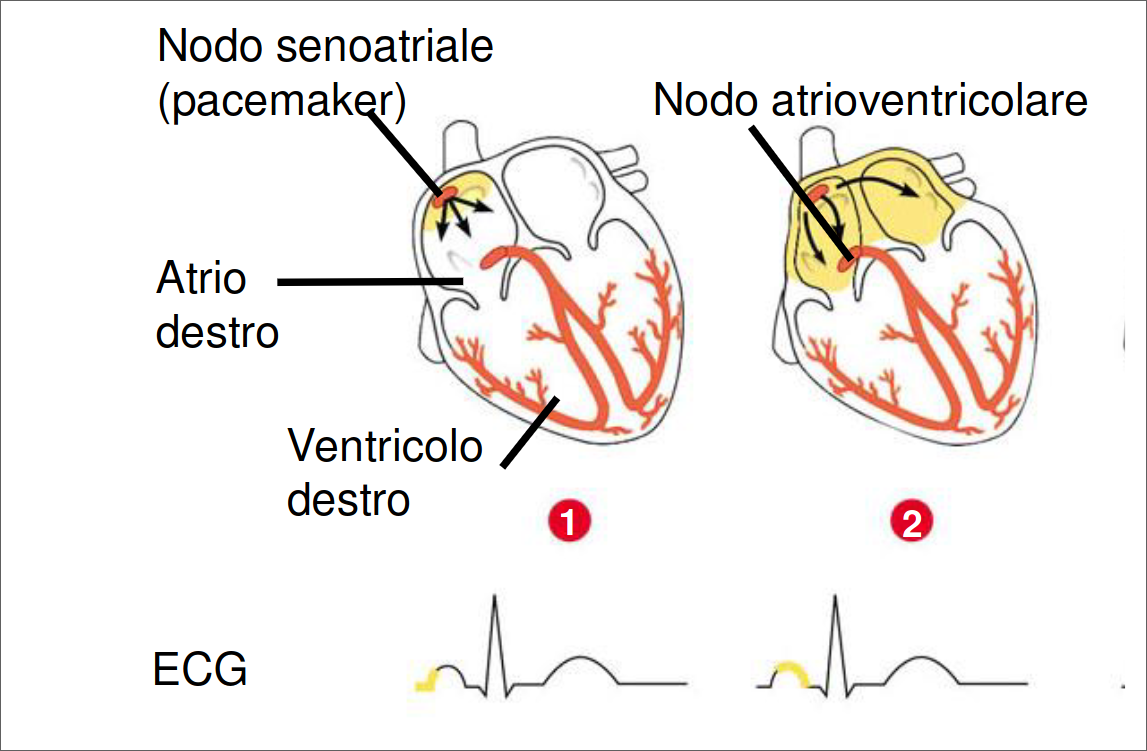
\includegraphics[width=0.9\textwidth]{./pacemaker.png}
\end{figure}
\end{center}

\pagebreak

\subsubsection{Circolazione coronarica}

\begin{center}
\begin{figure}[th]
    \centering
    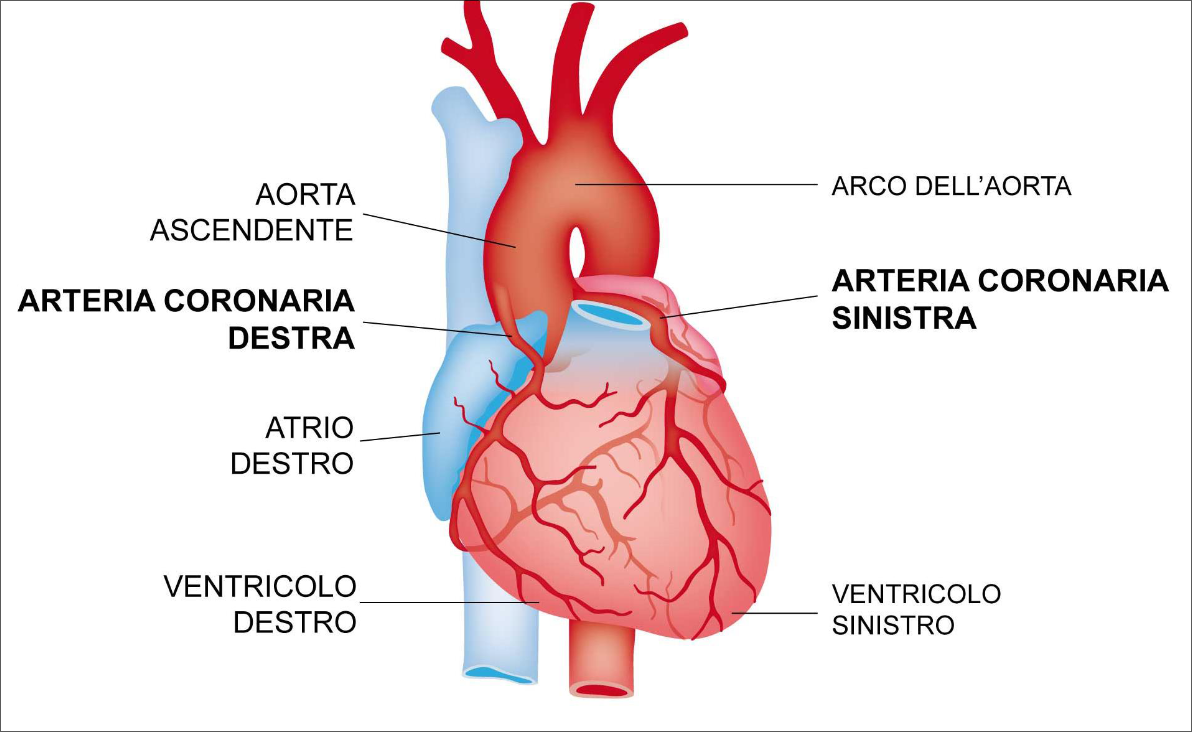
\includegraphics[width=0.7\textwidth]{./circolazione_coronarica.png}
\end{figure}
\end{center}

Le vene coronariche vanno ad alimentare il muscolo del cuore.

\subsubsection{Aterosclerosi}

\sdefinition{Ateroscelrosi}{
    L'\textit{ateroscelrosi} è una malattia che implica la formazione di placche (ateromi) all'interno delle pareti delle arterie.
}

Il lume si restringe e lo scorrimento del sangue diventa difficoltoso.
La causa principale è l'eccesso di colesterolo.

\subsubsection{Pressione sanguigna}

\sdefinition{Pressione sanguigna}{
    La \textit{pressione sanguigna} è la pressione esercitata dal cuore.
}

\setlength{\intextsep}{0pt}%
\begin{wrapfigure}{l}{8cm}
    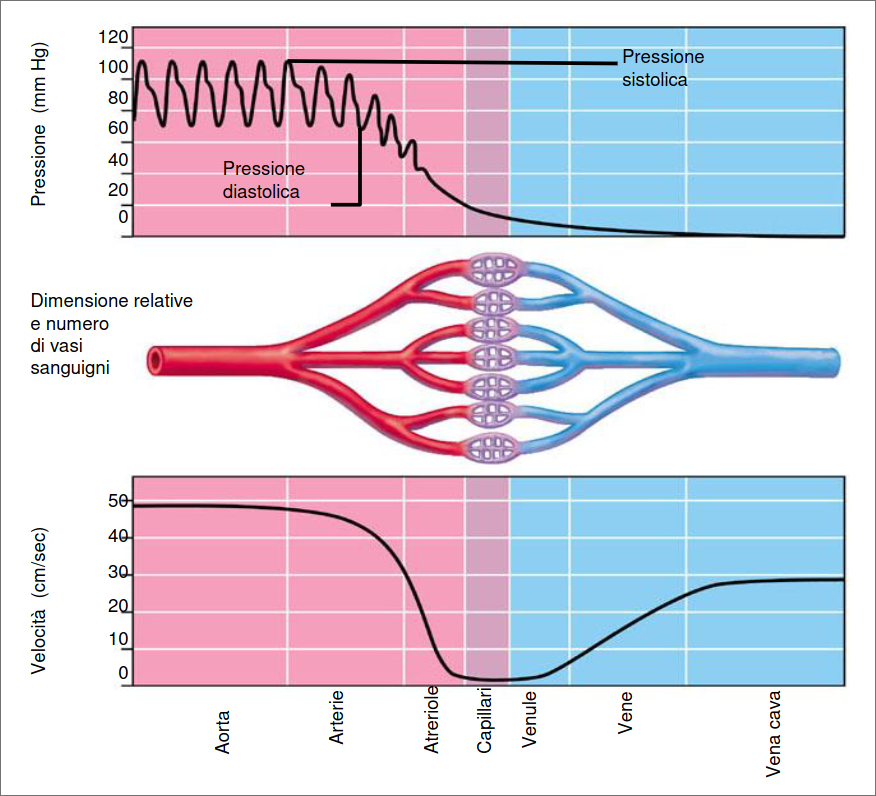
\includegraphics[width=7.5cm]{./pressione.png}
    \vspace{-1cm}
\end{wrapfigure}

La pressione sanguigna diminuisce più ci si allontana dal cuore, e diventa minima ai capillari.
Vi sono in realtà 2 pressioni:
quella sistolica (valore massimo, quando il ventricolo si contrae) e quella diastolica
(valore minimo, quando il vaso sanguignio si dilata e successivamente si richiude, dando una spinta).

Il valore normale della pressione sanguigna di un adulto è 120/70 (mmHg / mmHg).
Essa di misura con uno sfigmomanometro.

I muscoli scheletroci permettono al sangue di ritornare al cuore dopo i capillari.
Essi schiacciano il vaso spinegendo il sangue verso il cuore.
\wrapfill

\subsection{Il sistema respiratorio}

\subsubsection{Trasporto dei gas}

\begin{wrapfigure}{l}{0.525\textwidth}
    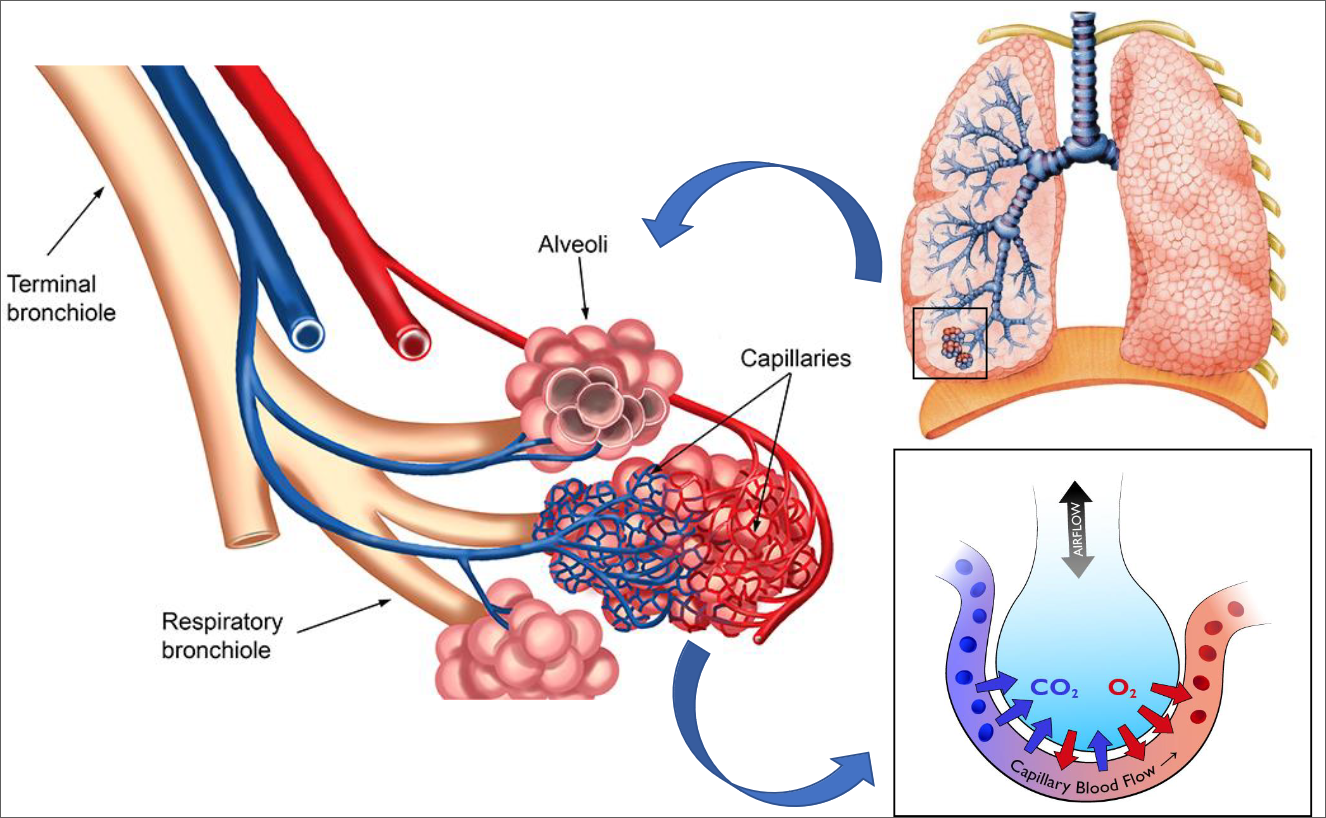
\includegraphics[width=0.5\textwidth]{./gas_transport.png}
    \vspace{-1cm}
\end{wrapfigure}

Gli scambi avvengono fra gli alveoli, dove avviene l'incontro fra il sistema
circolatorio e quello respiratorio.
I gas si muovono per diffusione semplice, e quindi passano fra i fosfolipidi (per gradiente di concentrazione).
Non è quindi possibile controllare la diffusione dei gas.

Una molecola di ossigeno deve trasversare 5 membrane per legare con l'emoglobina.

\wrapfill

\sdefinition{Pressione parziale}{
    La \textit{pressione parziale} (mmHg) corrisponde alla concentrazione di gas.
}

In tutti i vasi rossi la concentrazione di ossigeno è 100 mmHg, mentre in quelli blu è 40 mmHg.
\\
Nell'alveolo il gas rispecchia quello nell'ambiente circostante.
La concentrazione della cellula nei capillari è più bassa (40 o meno se sotto sforzo).

\subsubsection{Modalità di trasporto dell'ossigeno}

\begin{enumerate}
    \item Alla pressione parziale di pO\({}_2=100\) mmHG, presente nell'aria alveolare,
    solo 0.3 ml di O\({}_2\) (1.5\%) si sciolgono ogni 100 ml di sangue.
    \item La maggior parte dell'ossigeno (98.5\%), viene trasportato legato all'emoglobina.
    \item Per ogni globulo rosso ci sono 260 milioni di emoglobine.
\end{enumerate}

\subsubsection{Modalità di trasporto dell'anidride carbonica}

\begin{enumerate}
    \item Parte del CO\({}_2\) (5\%), viene trasportato disciolto nel plasma.
    \item Un'altra parte (5\%) si lega all'emoglobina.
    \item La maggior parte del CO\({}_2\) nel sangue (90\%) è trasportato nel plasma come ione bicarbonato. 
\end{enumerate}

Nel sangue dobbiamo avere una pH stabile, ma diossido di carbonio e acqua
si legano formando acido carbonico. Il globulo rosso spacca quindi questo acido,
tenendo lo ione idrone e rilasciando nel sangue solo lo ione bicarbonato.
Il bicarbonato torna CO2, il quale fuoriesce nei polmoni.
Ogni emoglobina può legare con 4 ossigeni.

\subsubsection{Curva di dissociazione dell'emoglobina}

\begin{figure}[ht]
    \centering
    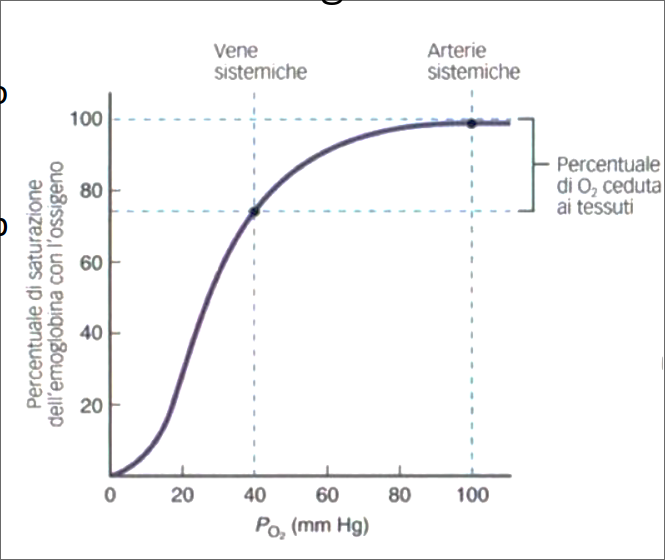
\includegraphics[width=0.65\textwidth]{./emoglobina.png}
\end{figure}

L'emoglobina lega con l'ossigeno in maniera non lineare.
La sua affinità nel legare con l'ossigeno dipende dalla concentrazione.

All'aumentare della PO2 la quantità di O2 che si lega all'Hb
prima aumenta rapidamente, poi tende a stabilizzarsi quando la saturazione si avvicina al 100\%.
Come mostra la tabella, alle normali pressioni parziali nelle
arterie e nelle vene sistemiche, a riposo, la percentuale di saturazione dell'Hb varia solo del 25\% circa.

Più le emoglobine sono legate con l'ossigeno, più è difficile che l'ossigeno si leghi con quelle rimanente,
e di conseguenza l'affinità dell'emoglobina è maggiore (vicino all'alveolo).

Vicino ai polmoni l'affinità è 100\%, mentre ai tessuri (40 mmHG), l'affinità è 75\%, per
cui 3/4 ossigeni per emoglobina.

Per sopravvivere ad un altitudine maggiore, dove l'ossigeno arriva ad una concentrazione del
75\%, l'affinità è comunque quasi 100\%. Di conseguenza, in alta montagna le emoglobine sono comunque
piene anche se la concentrazione dell'aria è minore.

\pagebreak

\subsection{Il sistema nervoso}

\sdefinition{Sistema nervoso}{
    Il \textit{sistema nervoso} è composto da una parte dell'encefalo (cervello), midollo spinale,
    nervi cranici e nervi spinali. Esso contiene prevalentemente neuroni.
}

Il midollo spinale fa parte del \textbf{sisema nervoso centrale} e sono quei neuroni
che passano nella colonna vertebrale.
Il \textbf{sistema nervoso periferico} sono quelli che portano tutte le informazioni che entrano
ed escono, ossia stimoli esterni e stimoli motori.

\begin{figure}[ht]
    \centering
    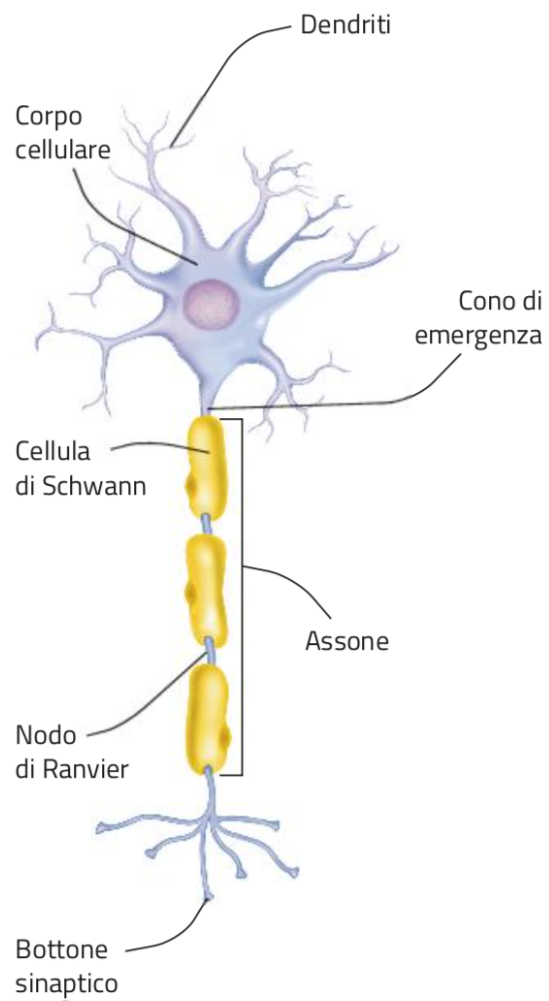
\includegraphics[width=0.75\textwidth]{./neuron.png}
\end{figure}

Le cellule del sistema nervoso che non sono neuroni si chiamano cellule gliali.
Esse sono più abbondanti dei neuroni e hanno svariate funzioni.
Vi sono le cellule
\begin{itemize}
    \item \textbf{di Schwann:} producono una sostanza isolante (mielina) che isola l'assone nel sistema nervoso periferico;
    \item \textbf{oligodendrociti:} producono una sostanza isolante (mielina) che isola l'assone nel sistema nervoso centrale.
\end{itemize}

La \textit{sinapsi} è il posto dove si scambia l'informazione fra il neurone presinaptico e postsinaptoco.

La differenza di potenziale nelle cellule dei neuroni è di -70 mV. Ogni cellula è caricata
negativamente data la minoranza di cariche positive al suo interno.
Tenere una differenza di potenzia necessita quindi ATP.

\subsubsection{Ventricoli, sostanza grigia e sostanza bianca nel SNC dei vertebrati}

\begin{figure}[ht]
    \centering
    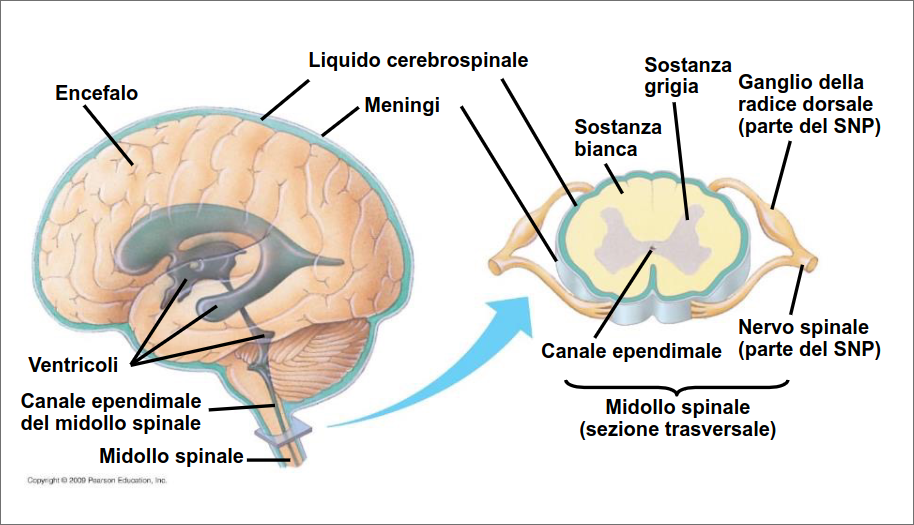
\includegraphics[width=0.75\textwidth]{./sostanza_grigia_bianca.png}
\end{figure}

Il midollo possiede una zona interna più scura (zona grigia), e una zona esterna più chiara
(zona bianca). Nella zone grigia abbiamo la maggior parte dei corpi cellulari,
mentre nella zona bianca abbiamo gli assoni.

L'effettore è quella parte che corpo che risponde allo stimolo.

Nel midollo ci sono risposte brevi e i segnali vengono elaborati solo minimamente per determinare se devono passare o meno.
Tutte le elaborazioni complesse vengono effettuate dall'encefalo.

Il sodio cerca di entrare perché c'è nè di meno all'interno, ma ce ne sarà di meno perché appena entra
viene buttato fuori dalla pompa.
Al contrario, il potassio cerca di uscire e la pompa lo ributta sempre all'interno.

% domanda esame: tutte le celle in ordine fra un segnale rosso che si vede in TV o il dito che cambia canale

\subsection{Trasmissione delle informazioni}

La trasmissione delle informazioni viene trasmessa mediante un impuslo elettrico
che viaggia in una sola direzione.

\sdefinition{Riflesso patellare}{
    Il \textit{riflesso patellare} è il riflesso spontaneo prodotto
    da uno stimolo sul ginocchio.
}

\vspace{0.5cm}

\begin{center}
\begin{figure}[ht]
    \centering
    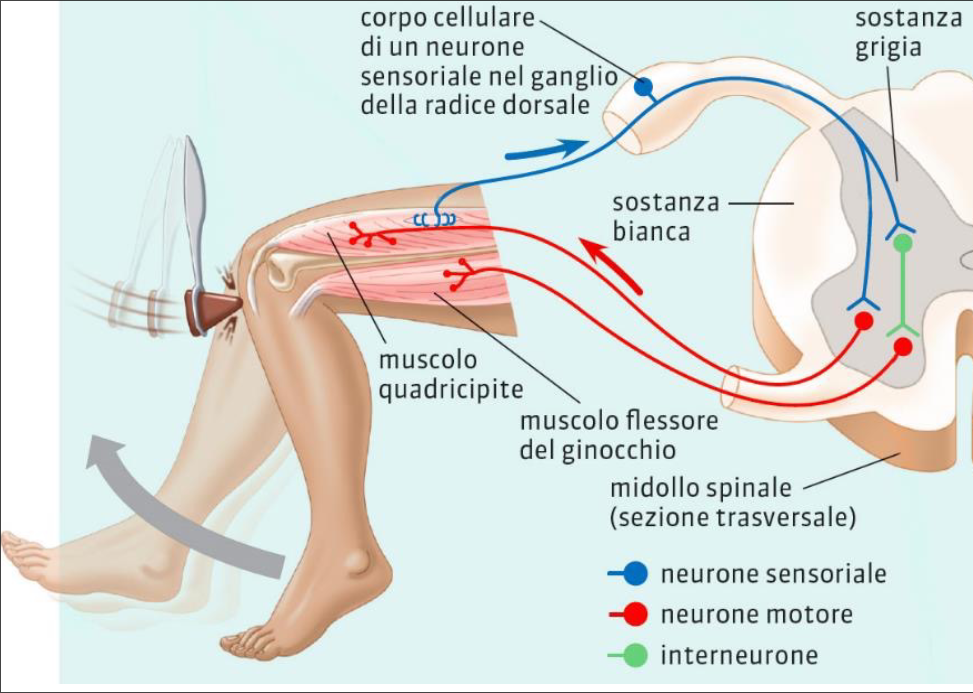
\includegraphics[width=0.75\textwidth]{./patellare.png}
\end{figure}
\end{center}

\subsection{La generazione del potenziale di riposo}

Anche in assenza di trasmissione, l'assione è pieno di ioni in movimento grazie alla pompa
sodio-potassio. Questa carica è chiamata potenziale di membrana,
e la cellula è caricata negativamente (potenziale di riposo).

In condizione di riposo, i canali sono chiusi, ma in caso di uno stimolo
i canali del sodio si aprono (la membrana si depolarizza leggermente).

Questo capovolgimento fa chiudere alla membrana il sodio e aprire il potassio.
La fuoriuscita del potassio riporta una carica negativa.
Questa successione di eventi è chiatamente potenziale di azione.

Quando la somma delle cariche sui dendriti supera una certa soglia (-50mV),
i canali si aprono e il segnale continua.

\sdefinition{Bottone sinaptico}{
    Bottone sinaptico è luogo dove si incontra il terminale pre sinaptico e i
    dendriti dei neuroni post sinaptici.
}

Se il canale si chiude, la differenza di potenziale lo fa aprire.
Di conseguenza, appena dopo essere stato chiuso (dopo un segnale), dovrebbe aprirsi nuovamente.
Questo provocherebbe l'espansione del segnale in entrambe le direzioni.
Infatti, questi canali del sodio vengono temporaneamente inibiti fino a che il segnale non è passato.

\textbf{Comunicazioni fra neuroni:}

\begin{itemize}
    \item  La \textit{sinapsi elettrica} è presente quado il segnale nervoso passa direttamente dal
    neurone presinaptico alla cellula successiva, detta postsinaptica (il bottone fonde con la cellula che viene dopo).
    \item La \textit{sinapsi chimica}
    \begin{itemize}
        \item Il neurone presinaptico secerne un neurotrasmettitore
        \item Il neurotrasmettire attraversa la fessura sinaptica
        \item Il neurotrasmettitore si lega ad un recettore sulla mebrana della cellula postsinaptica
    \end{itemize}
\end{itemize}

% pag 29
% TODO fessura sinaptica
% (3 stimola l'esocitosi)
% il calcio va alla vescicola e la fa fondere le vescicole contenenti trasmettori con la membrana (esocitosi, 4)
% escono i neurotrasmettitori nella fessura sinaptica
% il neurotrasmettori è una proteina
% essi derivano dal reticolo endoplasmatico rubido (sintetizzati da i ribosomi, poi trasportato nel golgi, e poi tutto il viaggio dal corpo del neurone fino alla sinapsi)

Quella elettrica è veloce ma non è modulabile.

I segnali possono essere eccitatori o inibitori.
Quelli eccitatori voglio far partire il segnale, mentre quelli inibitori
fermarlo. Quello che fa stato è il risultato, ossia la somma di tutte
all'inizio dell'assone.

\sdefinition{Seratonina}{
    La \textit{seratonina} è un neurotrasmettitore inibitorio.
}
Essa apre dei canali come quelli del potassio per inibire un determinato percorso.
L'inibizione di questo neurone postsinaptico è in un contesto che aiuta la felicità.

\pagebreak

\subsection{L'Occhio}

Gli occhi trasformano lo stimolo delle lunghezze d'onda della luce in segnali elettrici.
Questo processo si chiama trasfuzione sensoriale.

\vspace{0.5cm}

\begin{center}
\begin{figure}[ht]
    \centering
    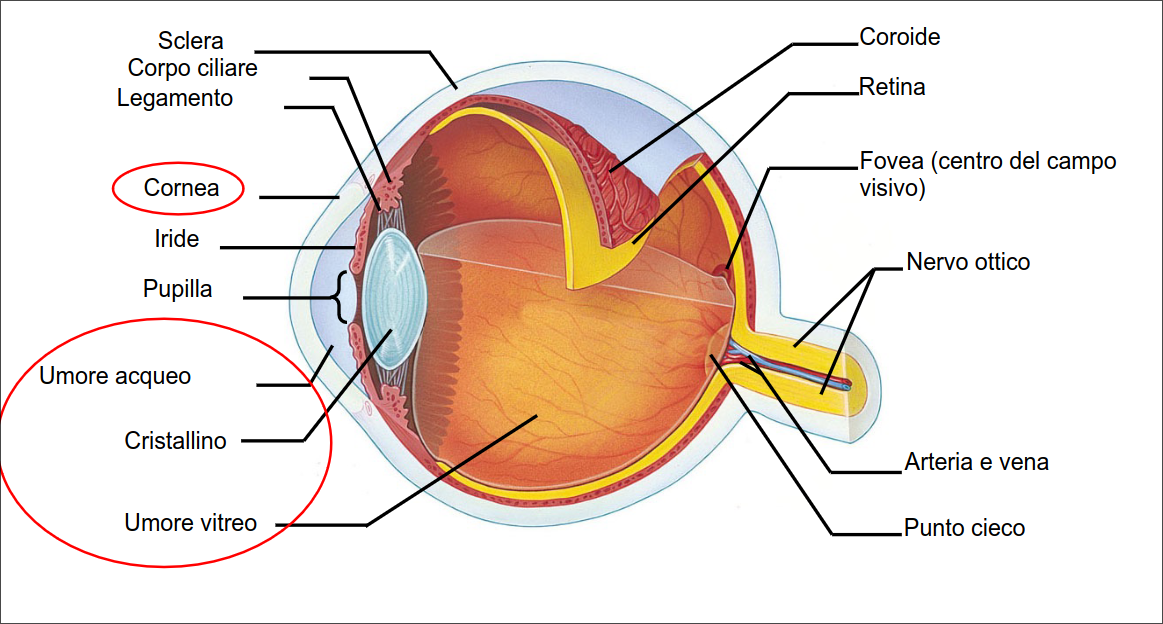
\includegraphics[width=0.9\textwidth]{./eye.png}
\end{figure}
\end{center}

Il nervo ottico trasporta gli impulsi elettrici verso il cervello.

\sdefinition{Sclera}{
    La \textit{sclera} costituisce la parte bianca protettiva dell'occhio.
}

\sdefinition{Retina}{
    La \textit{retina} è l'ultimo strato interno dell'occhio, dove la entra la luce.
    In questa zona vi sono i fotorecettori (recettori sensoriali) che captano lo sttimolo (lunghezza d'onda).
}

\sdefinition{Cornea}{
    La \textit{cornea} è una lenta che possiede una curva per deviare la luca, e farla atterrare in un punto preciso.
}

\sdefinition{Pupilla}{
    La \textit{pupilla} è il buco dove entra la luca. 
}

\sdefinition{Iride}{
    L'\textit{iride} è un muscolo con due funzioni
    \begin{itemize}
        \item regolazione del diametro della pupilla;
        \item blocco della quantità di luce in eccesso.
    \end{itemize}
}

La \textbf{fovea} è il punto centrale del campo visivo dove si trovano le cellule che si occupano di percepire i colori
Sul resto della retina, abbismo un altro tipo di cellule che capta solamente le tonalità (scuro / chiaro).

Il cristallino è una lente regolabile per mettere a fuoco un oggetto lontano o vicino
(per rimediare alla cornea che non è regolabile).

La luce viene quindi capovolta e proiettata in una determinata area.

Il punto dove entra il nervo ottico è detto punto cieco, sicocme non contiene ricettori.

L'umor acqueo è un liquido contenente nutrienti per dare nutrienti al resto dell'occhio.

\begin{center}
\begin{figure}[ht]
    \centering
    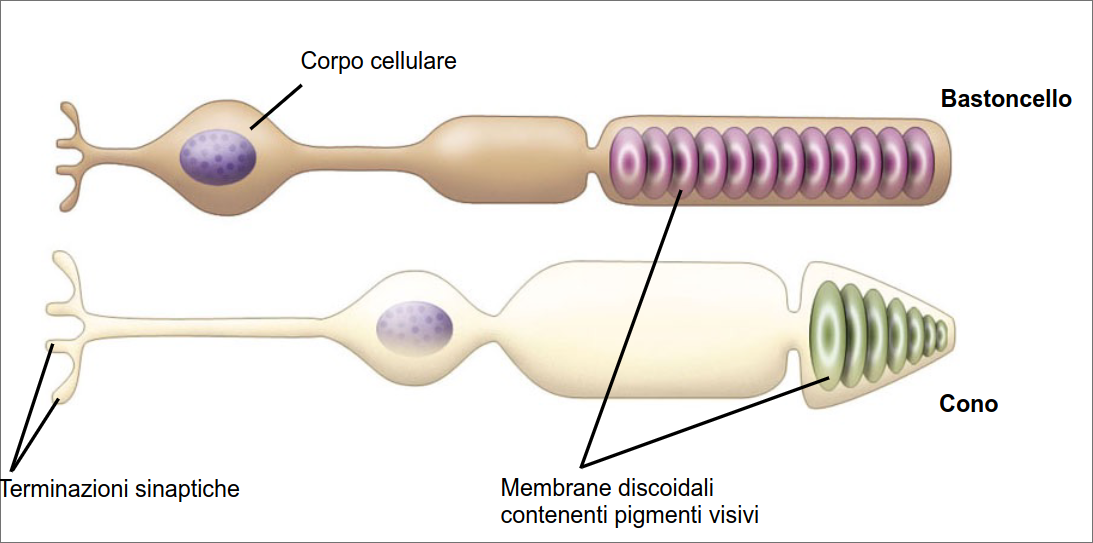
\includegraphics[width=0.8\textwidth]{./rods.png}
\end{figure}
\end{center}

Entrando il sodio la membrana depolarizza (dentro diventa più positivo).
Se la mebrana è depolarizzata, la cellula manda l'impulso.

\textbf{Foto bastoncelli al buio e alla luce:}

\begin{itemize}
    \item \textbf{Al buio:}
        Il livelli di cGMP sono elevati all'interno del citosol del segmento esterno
        del bastoncello, quindi i canali del sodio localizzati nella membrana del fotorecettore
        si aprono. Il sodio entra perché dentro la differenza di potenziale
        elettrico della cellula è negativo (gradiente elettrochimico).
        Gli ioni sodio entrano nella cellula e determinano una depolarizzazione
        (perché entrano cariche positive, dentro diventa più positivo, potenziale praticamente 0) che viaggia
        dal segmento esterno al terminale del fotorecettore. 
        In risposta alla depolarizzazione, si aprono i canali per il calcio.
        L'ingresso del calcio attiva un processo di esocitosi che porta al rilascio del neurotrasmettitore.
        Il neurotrasmettitore agisce sulle cellule bipolari, generando dei potenziali graduati (le blocca non facendole scaricare)
    \item \textbf{Alla luce:}
        Se c'è luce il pigmento cambia forma. I livelli di cGMP nel citosol del segmento esterno diminuiscono, quindi i canali del sodio si chiudono.
        Il minore ingresso di sodio iperpolarizza la cellula (potenziale negativo all'interno),
        a causa dell'uscita del potassio.
        L'iperpolarizzazione provoca la chiusura dei canali del calcio nel segmento interno,
        quindi viene rilasciato meno neurotrasmettitore dal terminale del fotorecettore.
        La cellula bipolare quindi non riceve nessun segnale, è attiva e quindi scarica
        e di conseguenza anche la gangliare.
\end{itemize}

\pagebreak

\section{Biologia cellulare e genetica}

\subsection{Replicazione}

\sdefinition{Mitosi}{
    La \textit{mitosi} consiste nella duplicazione completa di una cellula.
}
Nella cellula eucariota umana il DNA è diviso in 46 filamenti, chiamati cromosomi.
Prima di fare la mitosi è essenziale duplicare il materiale genetico, ossia il DNA.
La mitosi può produrre solo cellule \textbf{somatiche}.

Per quel che concerne la riproduzione sessuale,
avviene la \textbf{meiosi}, che produce cellule \textbf{germinali}
(ossia spermatozoi e ovuli), chiamati gameti.
Essi contengono solamente 23 cromosomi ciascuno.

La fecondazione è il processo di incontro fra ovulo e spermatozoo,
dove il numero di cromosomi si somma.
I 46 cromosomi sono in realtà 23 coppie, ogni coppia con una componente dal padre e uno dalla madre.

\sdefinition{Zigote}{
    Lo \textit{zigote} è la prima cellula prodotta dalla fecondazione.
}
Eseguendo la mitosi, lo zigote si duplica in \(2^n\) cellule.

\sdefinition{Aploidi}{
    Con \textit{aploide} si intende una cellula con solo un set (23) di cromosomi.
}
Ovuli e spermatozoi sono aploidi.

\sdefinition{Diploide}{
    Con \textit{diploide} si intende una cellula con 23 coppie (46) cromosomi.
}
Due cellule aploidi formano due cellule diploidi.

Le uniche cellule che fanno la meiosi sono le cellule diploidi nei testicoli e nelle ovaie.

\sdefinition{Cromosomi omologhi}{
    I cromosomi appartenenti ad una coppia di cromosomi con gli stessi geni vengono detti
    \textit{cromosomi omologhi}.
}

La meiosi consiste nel separare tutti i cromosomi omologhi per averne 23.
La meiosi crea 4 cellule, mentre la mitosi 2.

\subsection{Cellule staminali}

\sdefinition{Cellula staminale}{
    Con \textit{cellula staminale} si intende una cellula non specializzata,
    capace di differenziarsi specializzandosi in uno dei molti tipi di cellule
    diverse presenti nel nostro corpo.
}
Le cellule staminali sono le cellule che si specificano.

\subsection{Processi della facoltà eucariota}

Le funzioni principali di una cellula eucariota possono essere:

\begin{itemize}
    \item mitosi;
    \item meiosi;
    \item sopravvive (nutrimento, respirazione);
    \item essere uccisa (es. dal sistema immunitario);
    \item morire (anche suicida, apoptosi);
    \item svolge la propria mansione;
    \item mutare (diventare cancerogena).
\end{itemize}

\subsection{Genetica}

\sdefinition{Locus gnetico}{
    Con \textit{locus genetico} si intende si intende una posizione fissata per
    un certo gene nel cromosoma.
}

Le varianti di un gene si chiamano \textbf{alleri}, i quali possono essere uguali o diversi
(es. occhi marroni-verdi etc.). Per ogni gene vi sono 2 alleri, siccome vi è una coppia di cromosomi omologhi.

\sdefinition{Cromatina}{
    la \textit{cromatina} è il DNA composta da 46 cromosomi singoli non spiralizzati (formano un groviglio).
}

Durante la duplicazione del DNA, all'interno della cromatina,
alcuni enzimi duplicano tutti i cromosomi.
I 92 cromosomi nella cromatina vengono separati correttamente, rimanendo non spiralizzati.
Successivamente i cromosomi si spiralizzando su delle proteine formando una struttura spiralizzata ad X.
% immagine

\sdefinition{Cromatidi}{
    I \textit{cromatidi} sono le braccia di un cromosoma X.
    Un cromosoma X ha quindi 2 cromatidi fratelli (destra e sinistra).
}

La mitosi consiste nel separare i cromatidi fratelli, e quindi duplicare l'informazione,
ottendo due cromosomi singoli spiralizzati.

\sdefinition{Cariotipo}{
    Con \textit{cariotipo} si intende l'insieme di tutti le 23 coppie di cromosomi. % rivedere Def
}

Gli ultimi due cromosomi sono quelli che determinano il sesso (cromosomi sessuali),
mentre gli altri si chiamano \textbf{autosomi}.

\begin{center}
\begin{figure}[ht]
    \centering
    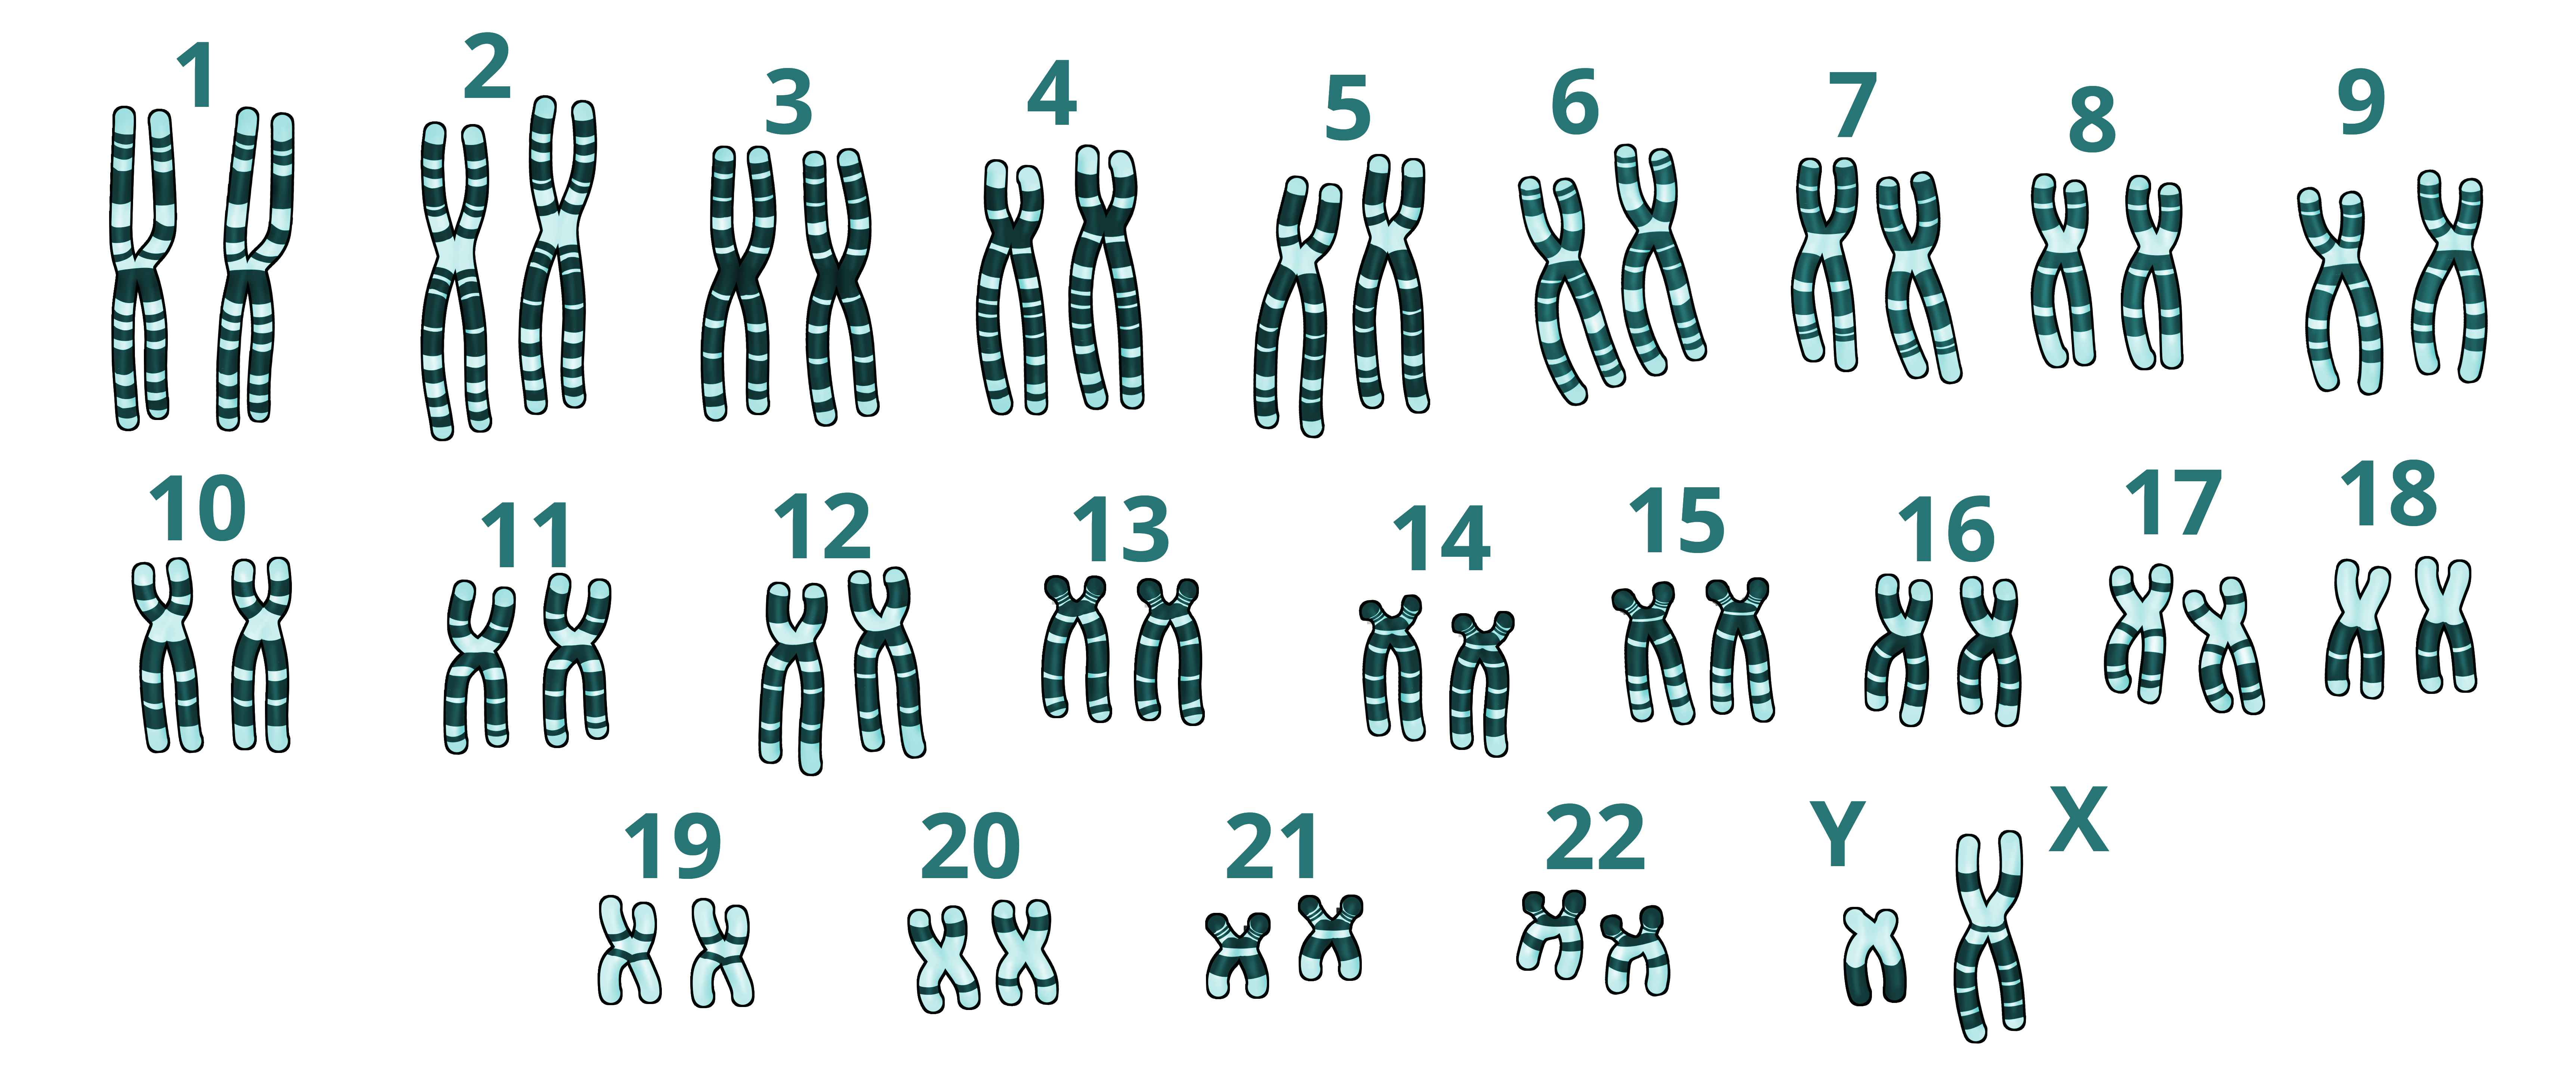
\includegraphics[width=0.8\textwidth]{./cariotipo}
\end{figure}
\end{center}

\subsection{Ciclo cellulare}

\vspace{0.1cm}

\begin{center}
\begin{figure}[ht]
    \centering
    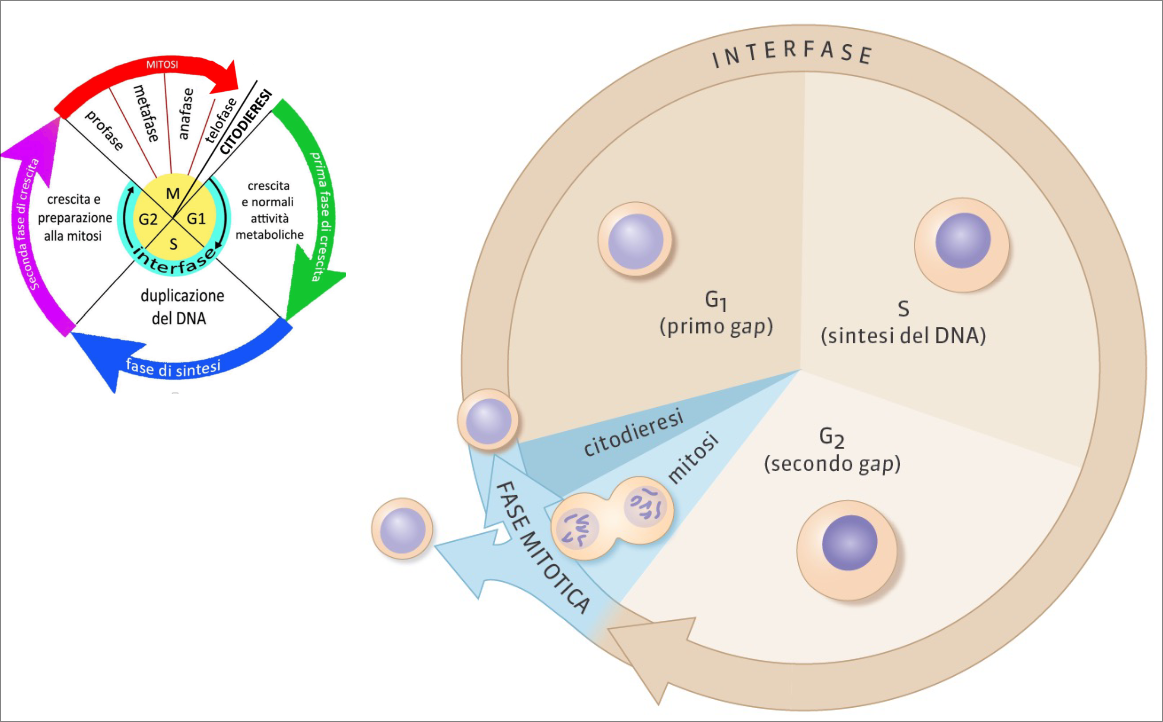
\includegraphics[width=\textwidth]{./ciclo_cellulare}
\end{figure}
\end{center}

Nella fase g1 la cellula non fa nulla e continuano la loro vita svolgendo le loro funzioni metaboliche. 
Le cellule staminali o quelle che diventano gameti entrano nella fase S in cui il DNA viene duplicato. 
Nella fase G2 la cellula si prepara alla divisione, e inizia a spiralizzare la cromatina. 
Tutto ciò si chiama interfase.
Nella fase mitotica la cellula viene divisa nella mitosi e quanto tutto è separato si taglia e si hanno due cellule separate, questa fase si chiama citodieresi.

\begin{center}
\begin{figure}[ht!]
    \centering
    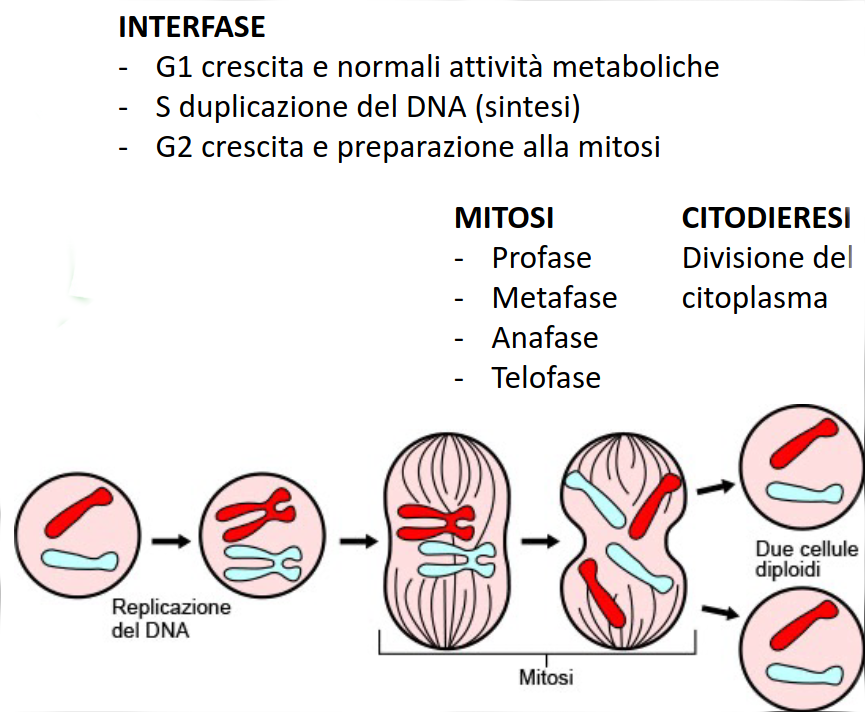
\includegraphics[width=0.6\textwidth]{./ciclo_cellulare2}
\end{figure}
\end{center}

Nella realtà la cromatina non contiene i cromosomi spiralizzati, a differenza del disegno.

Il ciclo della cellula è controllato in base all'ambiente esterno.
Se la cellula è sana e vi è nutrimento, la cellula può andare in mitosi.
Vi sono quindi tre controlli o checkpoint che bloccano il passaggio ad una fase ulteriore
se le condizioni non sono rispettate.
Le cellule cancerogene eludono questi checkpoint.

\begin{center}
\begin{figure}[ht]
    \centering
    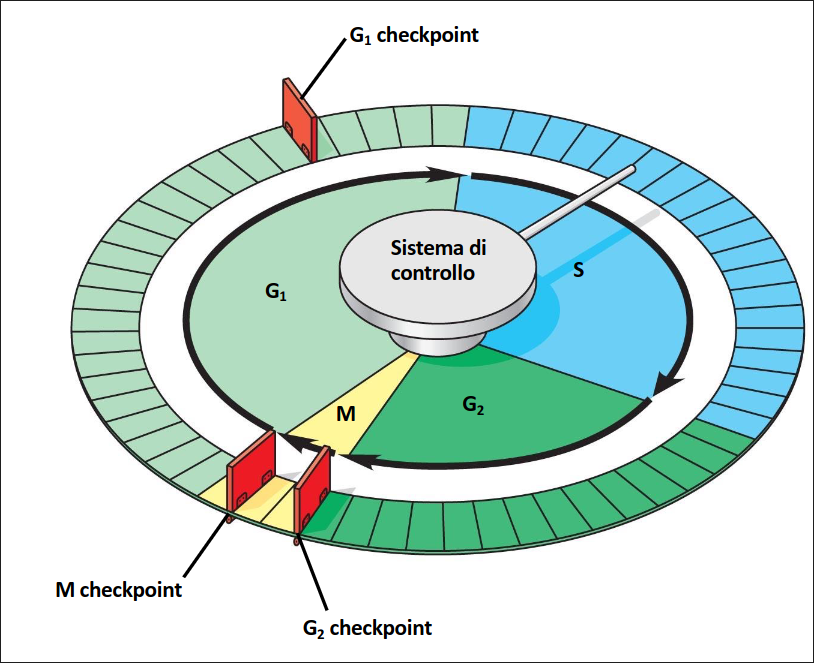
\includegraphics[width=0.75\textwidth]{./ciclo_cellulare3}
\end{figure}
\end{center}

Se la cellula diviene differneziata resterà sempre in G\({}_0\).
\\
Il DNA, durante tutta l'interfase, è sotto forma di cromatina nel nucleo.
Durante la fase S dell'interface, inizia la duplicazione.
Si creano delle bolle di duplicazione sui cromosomi, formando
coppie di cromosomi omologhi duplicati (I cromosomi omologhi sono incollati fra di loro).
Ogni cromosoma duplicato ha due cromatidi fratelli che sono assolutamente identici.
In mitosi abbiamo solo a che vedere con cromosomi spiralizzati.
I due cromatidi fratelli, appena staccati, diventano cromosomi e si posizionano in cellule diverse.

Prima della meiosi e mitosi, vi è la medesima situazione: 46 cromosomi omologhi duplicati.
Nella metafase della mitosi, i 46 cromosomi sono uno in fila all'altro,
mentre nella meiosi si mettono a coppie uno in fila all'altro (per cui 23 coppie in fila).

\sdefinition{Tetrade}{
    Nella metafase della meiosi, le coppie di cromosomi omologhi vengono chiamate
    \textit{tetradi}.
}

\vspace{0.25cm}

\begin{center}
\begin{figure}[ht]
    \centering
    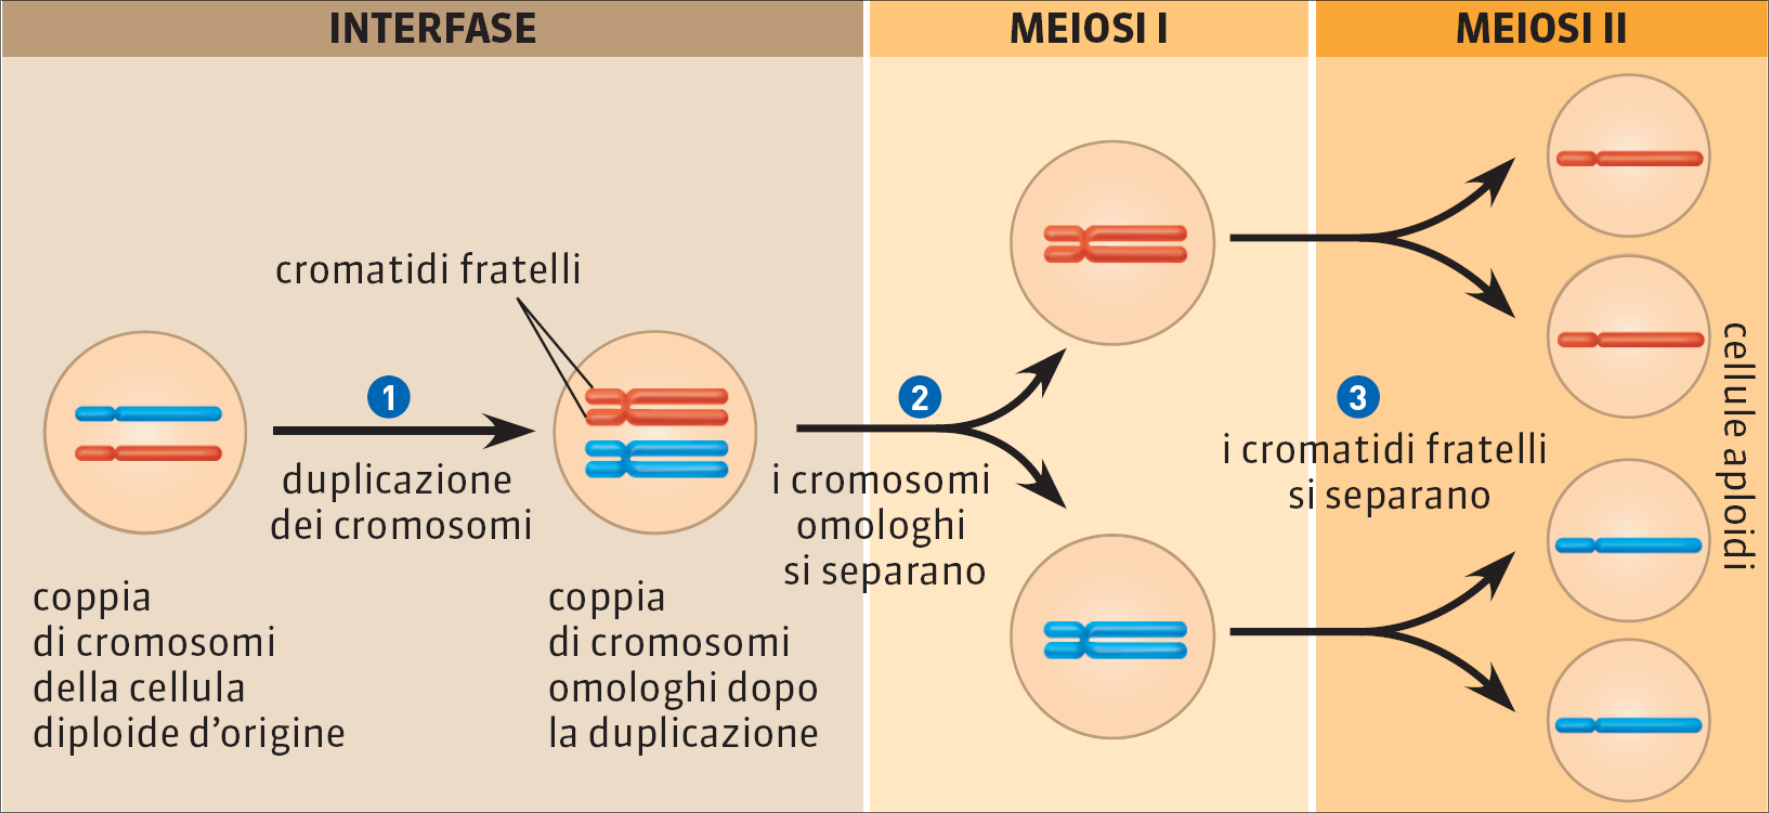
\includegraphics[width=0.75\textwidth]{./meiosi_schema}
\end{figure}
\end{center}

% Schema MITOSI / MEIOSI giallo e violaceo
% Importantissimo da sapere tutto esattamente!!
% Meglio "duplicazione del materiale genetico" al posto di "duplicazione dei cromosomi"

I tumori hanno origine da mitosi mal riuscite.

\subsubsection{Problemi della mitosi}

\sdefinition{Trisomia 21}{
    La \textit{trisomia 21} è un disturbo per quale vi è un cromosoma extra (il cromosoma 21).
}

\begin{center}
\begin{figure}[ht]
    \centering
    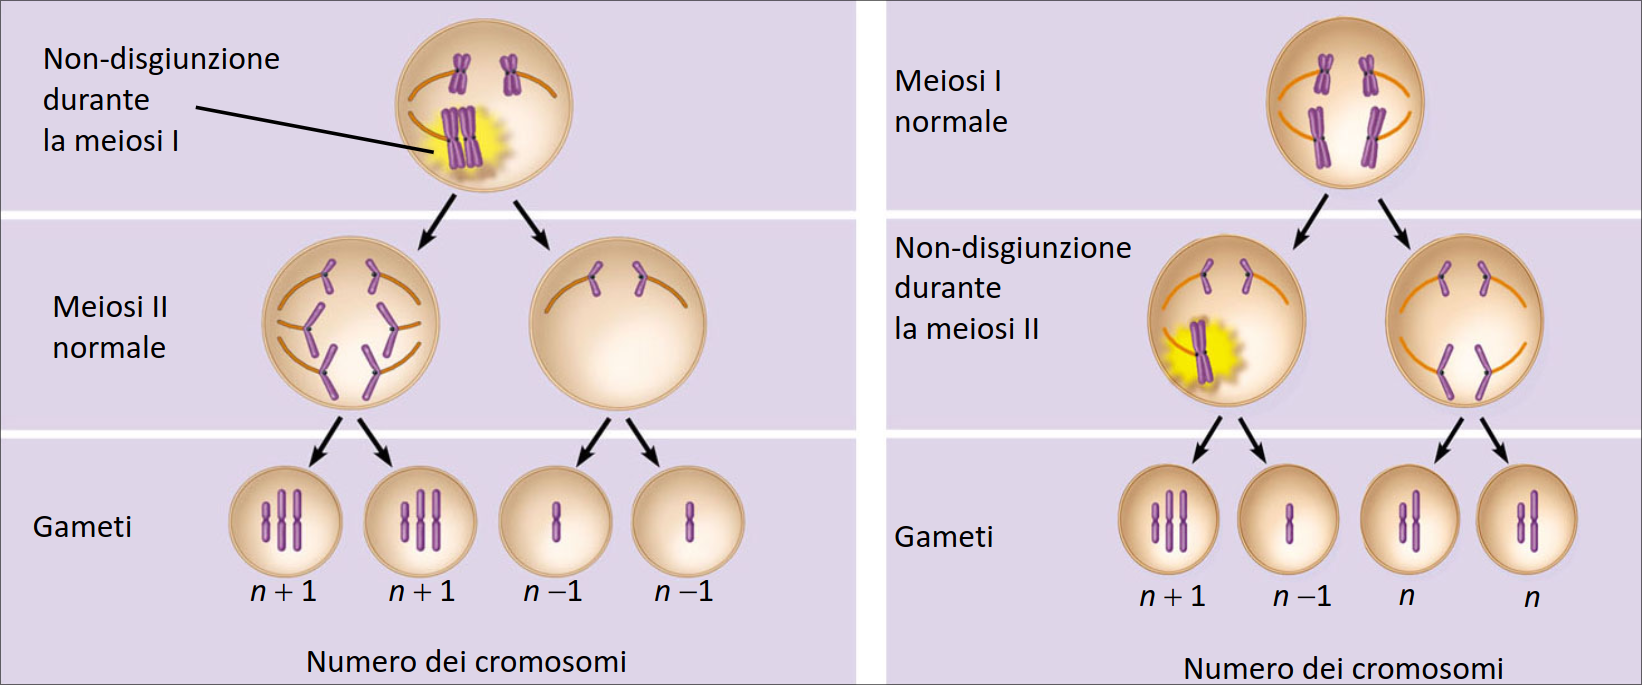
\includegraphics[width=0.75\textwidth]{./trisomia21}
\end{figure}
\end{center}

% TODO spiegare lo schema
La motivazione più comune è data dalla madre, dove l'indice di rischio aumenta
esponenzialmente dopo i 35 anni.
Usando ovuli vecchi (gli ovuli sono prodotti alla nascita e rimangono gli stessi),
è più probabile che i cromosomi non si stacchino.

\pagebreak

\subsection{La riproduzione negli esseri viventi}

\sdefinition{Riproduzione}{
    La \textit{riproduzione} è un processo per il quale viene data origine ad uno o più organismi
    discendenti.
}

\sdefinition{Riproduzione asessuata}{
    La \textit{riproduzione asessuata} non coinvolge l'impiego di cellule specializzate (gameti),
    e consiste nel clonarsi in maniera identica.
}
La riproduzione asessuata è veloce, non necessita un secondo individuo ma
produce poca variabilità genetica.

\sdefinition{Riproduzione sessuata}{
    La \textit{riproduzione sessuata} coinvolge due individui di sesso opposto per produrre un discendente
    con una varietà genetica.
}
La riproduzione sessuata si avvale di mutazioni genetiche.
Essa costa molta più energia, è lenta, richiede due individui di sesso opposto ma
genera una grande diversità genetica.

\pagebreak

\section{Esercizi}

\sexercise{Qual'è il polimero di glucosio che permette agli esseri umani una riserva energetica?}{
    Il glicogeno.
}

\sexercise{In che modo l'ossigeno gassoso riesce ad entrare nel sistema cardiocircolatorio e raggiunge i mitocondri dei muscoli degli arti inferiori? Spiega sul piano anatomico e fisiologico}{
    L'ossigeno entra nell'apparato respiratorio.
    L'ossigeno viene inserito nel globuli rossi passando per l'alveolo.
    Un po' di ossigeno viene disciolto nel sangue piuttosto che nel globulo rosso.
    I globuli rossi vengono trasportati dal sangue fino alle cellule di tutto il corpo.
    L'ossigeno, la quale è una molecole piccola, raggiunge il mitocondrio mediante una diffusione semplice (per gradiente) per cui trasporto passivo semplice.
}

\sexercise{Spiega come avviene la condensazione di due amminoacidi in una cellula umana, specificando i dettagli molecolari}{
    Due monomeri di proteine si uniscono mediante la condensazione, la quale libera una molecola di acqua.
    All'interno della cellula, ciò avviene quando un gruppo \(O\) si incontra con il gruppo \(OH\) dell'altro monomero.
}

\sexercise{È possibile definire un mitocondrio all'interno di una cellula un sistema vivente? Spiega e argomenta}{
    Sì, perché il mitoconfrio è autopoietico e può riprodursi da solo.
}

\sexercise{Degli anticorpi (proteine) sono stati prodotti dal sistema immunitario (cellule bianche) per contrastare un'infezione virale nel lume intestinale. In che modo queste proteine possono raggiungere tale luogo?}{
    Una volta prodotti, gli anticorpi vengono rilasciati nel flusso sanguigno e circolano in tutto il corpo. Essi sono in grado di raggiungere qualsiasi parte del corpo attraverso il sistema circolatorio.
    Per raggiungere il lume intestinale e combattere un'infezione virale in quella zona, gli anticorpi devono attraversare la barriera mucosale dell'intestino. Questa barriera mucosale è costituita da uno strato di muco e cellule epiteliali. Gli anticorpi non possono semplicemente passare attraverso questa barriera a meno che non siano specifici per l'infezione virale nell'intestino.
    per esocitosi esce dalla cellula della parete del vaso, per endocitosi entra nella parete dell'intestino, e per esocitori viene buttato fuori nel lume intestinale.
}

\sexercise{Dove vengono interpretati gli impusli elettrici provenienti dall'occhio?}{
    Zona logocipitale, nella parte posteriore della corteccia celebrare.
}

\sexercise{Come fa l'occhio a mettere a fuoco un oggetto vicino?}{
    Mediante il processo di accomodamento/accomodazione.
}

\sexercise{Come si chiamano i due tipi principali di fotorecettori?}{
    Coni e bastoncelli.
}

\sexercise{Come mai la pupilla è nera?}{
    La pupilla ha il colore dato dall'iride,
    grazie al nero tutti i colori vengono assorbiti.
}

\end{document}

Gradiente elettrochimico:
- Combinazione del gradiente di concentrazione e del potenziale elettrico attraverso la membrana
- Condiziona trasporto attivo e diffussione facilitata finluenzando la direzinoe e l'efficienza/velocità del movimento delle molecole.
- Movimento dipende da carica molecole e da differenza di potenziale/differenza di carica elettrica tra interno ed esterno.


Fermentazione:
- Generazione di ATP
- Rigenerazione di coenzimi NAD+
- Eliminazione di piruvato

=========
L'energia data in un organismo è data dalla differenza
di energia spesa per spaccare legami e i nuovi legami che si formano, che sono inevitabilmente pi?u stabili